\documentclass[12pt]{article}
%\usepackage[utf8]{inputenc}
%\documentclass[UTF8]{ctexart}
%\usepackage[UTF8, heading = false, scheme = plain]{ctex}
\usepackage{geometry}
%geometry{a4paper,scale=0.9}
\geometry{a4paper,left=1cm,right=1cm,top=1cm,bottom=2cm}
\usepackage{amsfonts}
\usepackage{color}
\usepackage{url}
%\usepackage{biblatex}
\usepackage{amsmath}
\usepackage{amssymb}
\usepackage{latexsym}
\usepackage{cite}
%\addbibresource{ref.bib}
%\bibliography{ref.bib}
\usepackage{caption}
\usepackage{graphicx, subfig}
\usepackage{float}
%\usepackage[fontset=ubuntu]{ctex}
%\usepackage{fontspec}
\usepackage{xeCJK}
%\usepackage[colorlinks,
%anchorcolor=black,
%citecolor=black]{hyperref}
%\setmainfont{SimSun}
\usepackage[section]{placeins}
\usepackage{enumitem}
\usepackage{framed}
\usepackage[framemethod=TikZ]{mdframed}
\usepackage{indentfirst}
\usepackage{setspace}%使用间距宏包
\linespread{1.5}

\title{群论基础总结\cite{From_Linear_Equation_To_Galois_Theory}\cite{Visual_Group_Theory}}
\author{leolinuxer}
%\date{June 2020}

\begin{document}
%\setlength{\parindent}{0pt}
\maketitle
\tableofcontents

\section{集合与映射}
\subsection{集合基本概念}
\begin{itemize}
\setlength{\itemsep}{0pt}
\setlength{\parsep}{0pt}
\setlength{\parskip}{0pt}
    \item \textbf{并集}:$C = A\cup B$,即$x\in C \Leftrightarrow x\in A \quad or \quad x \in B$
    \item \textbf{交集}:$C = A \cap B$,即$x\in C \Leftrightarrow x\in A \quad \& \quad x \in B$
    \item \textbf{差集}:$C = A - B$,即$x\in C \Leftrightarrow x\in A \quad \& \quad x \notin B$
    \item \textbf{直积}:$C = A \times B = \{(a,b)|a\in A \& b \in B\}$
\end{itemize}

若映射$f: A \rightarrow B$有如下不同情况,可以区分出:

1) 若$A \subset B$,而$f$满足$f(a) = a, \forall a \in A$,则称$f$为\textbf{包含映射},记为$i$;若此时 $B=A$,此时的 $i$ 称为$A$的\textbf{恒等映射},记作$1_A$。

2) 若$f(A) = B$,则称$f$为\textbf{$A$到$B$的满射}

3) 若 $f(a) = f(a') \Rightarrow a = a', a,a \in A$,则称 $f$ 为\textbf{单射}。

4) 若$f$ 既是单射又是满射,则称$f$为\textbf{双射};此时从 $f(a) = b$,可记$a = f^{-1}(b)$,从而确定了映射$f^{-1}: B \rightarrow A$,称为$f$的\textbf{逆映射}。

5) 若$C \subset A$,则由于$f(c) \in B$ 对应于$c \in C$,可定义$f_c: C \rightarrow B$,即把$f$的定义域缩小到$C$上,则称$f_c$为$f$到$C$的\textbf{限制}。
\begin{figure}[H]
    \centering
    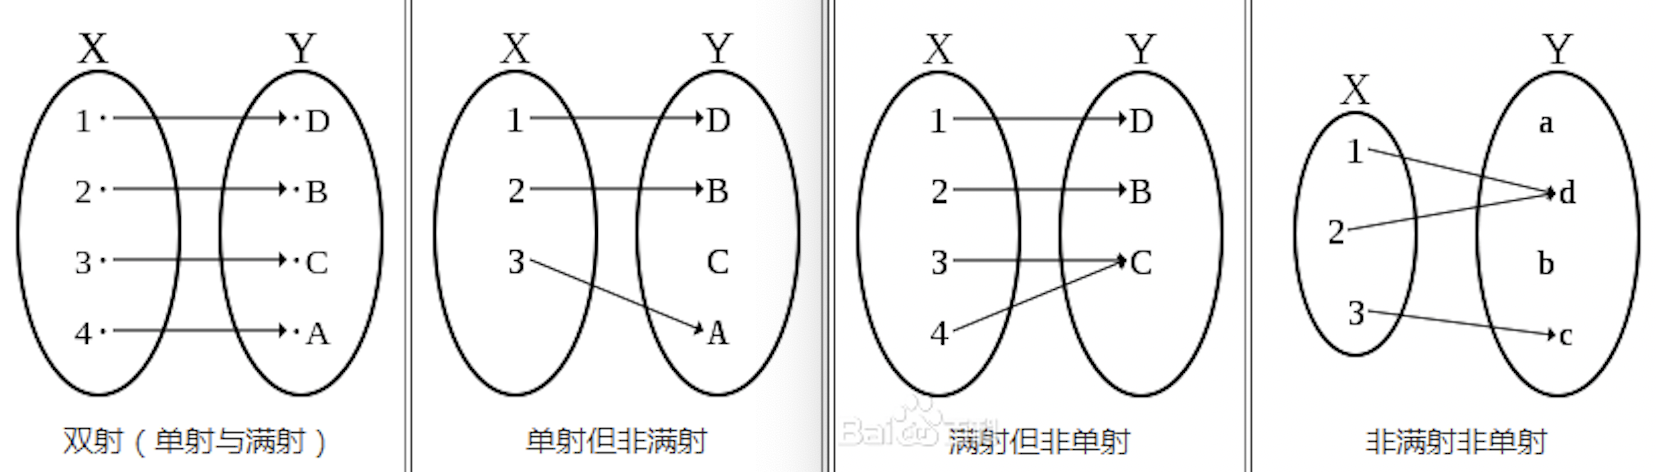
\includegraphics[width=.8\textwidth]{fig/SetMappingClassification.png}
\end{figure}

\begin{framed}
%\verb|\documentstyle[ifthen,12pt,titlepage]{article}|
\small{
如果$f: A \rightarrow B$,且$g: B \rightarrow C$,此时把$a \in A$映为$h(a) = g(f(a)) \in C$ 来定义映射$h: A \rightarrow C$,则称$h$为$f$和$g$的\textbf{结合},记作$h = g\circ f$

如果$f: A \rightarrow B$是双射,不难看出$f^{-1}: B \rightarrow A$也是双射,且 $f^{-1}\circ f = 1_A, f\circ f^{-1} = 1_B$

对于$f: A \rightarrow B, g: B \rightarrow C, h: C \rightarrow D$,有$h\circ (g\circ f) = (h\circ g)\circ f$,即映射的结合运算满足结合律。
}
\end{framed}

\subsection{集合的等价关系和分类}
“映射”反应的是一个集合与另一个集合的外部联系;\textbf{“关系”}给出了集合内元素的内部联系。

集合上的一个\textbf{关系$\sim$},指的是一种法则。由它可以判断任意$a,b\in A$所构成的有序偶$(a,b)$ 是满足某种条件(此时称$a,b$有关系,记作$a\sim b$),还是不满足这一条件(此时称$a,b$无关系,记作$a\nsim b$)

\begin{framed}
%\verb|\documentstyle[ifthen,12pt,titlepage]{article}|
\small {
例如大于($\ge$)就给出了整数集合$Z$的一个关系;对于三角形的集合,三角形的全等和相似也分别给出了这个集合的一个关系。
}
\end{framed}

\subsubsection{等价关系}
集合$A$上定义的关系$\sim$,若满足如下条件,则称$\sim$是一个等价关系:

1) 自反律:对$\forall a \in A \Rightarrow a \sim a$

2) 对称率:对$a \sim b \Rightarrow b \sim a$

3) 传递率:对$a \sim b, b \sim c\Rightarrow a \sim c$


\subsubsection{集合的分类}
集合$A$的一个\textbf{分类},指的是把$A$分成许多称为\textbf{类}的非空子集合$A_a, A_b, \cdots $,而其中每两个不同类的交集为空集,它们全体的并集是$A$。

设$\sim$是集合$A$的一个等价关系,对于$a\in A$,我们把$A$中所有与$a$等价的元都汇集在一起,而构造出$A$的子集合$A_a$,如果此时存在$b \in A$,且 $b \notin A_a$,则同样构造$A_b$,显然这些$A_a, A_b, \cdots $给出$A$的一个分类。

反过来,如果给定了$A$的一个分类,那么我们就可以如下的定义$A$的一个等价关系:$\sim: a \sim b$,当且仅当$a,b$属于同一类;$a \nsim b$,当且仅当$a,b$不属于同一类;

总结后有:集合$A$的一个分类可以确定它的一个等价关系;反之,集合$A$的一个等价关系可以确定它的一个分类。

因此,类也称为\textbf{等价类}。而$A_a$称为\textbf{由$a$确定的等价类}, $a$是$A_a$的一个\textbf{代表}。当然,若$a \sim b$,则$A_a = A_b$,即一个等价类可以由其中的任一元做代表,因为有这种随意性,所以任何关于等价类的命题首先必须与\textbf{代表元的选取无关}。

\begin{framed}
%\verb|\documentstyle[ifthen,12pt,titlepage]{article}|
\small {
全体奇数和全体偶数这两个集合构成了整数集合$Z$的一个分类。

理解:集合的分类是\textbf{不重不漏}的。
}
\end{framed}

\subsection{商集合}
由$A$的等价关系$\sim$,确定了$A$的各个类$A_a, A_b, \cdots$,以这些类做为元素而得到的集合,称为由$A$按$\sim$而确定的商集合,记作:
$$
A / \sim = \{A_a, A_b, \cdots \}
$$

此时,很自然的由$a$对应$A_a$,可定义$f: A \rightarrow A/\sim$,容易验证这是一个满射,称为$A$到商集合$A/\sim$上的\textbf{自然映射}。

\section{群简介}
\subsection{魔方的例子}
考虑一下魔方的特点:
\begin{itemize}
\setlength{\itemsep}{0pt}
\setlength{\parsep}{0pt}
\setlength{\parskip}{0pt}
    \item 预先定义了一组基本“动作”(这些基本的“动作”,叫做群的\textbf{“生成元”,generator})
    \item 每一个“动作”都是可逆的
    \item 每一步“动作”都是确定性的(“动作”之后的结果是可预测的)
    \item 任何一组连续的“动作”序列,也是一个“动作”。
\end{itemize}

\subsection{群定义}
\begin{mdframed}[
linecolor=black!40,outerlinewidth=1pt,roundcorner=.5em,innertopmargin=1ex,innerbottommargin=.5\baselineskip,innerrightmargin=1em,innerleftmargin=1em,backgroundcolor=gray!5,
%backgroundcolor=blue!10,%userdefinedwidth=1\textwidth,%shadow=true,%shadowsize=6,%shadowcolor=black!20,%frametitle={The \textit{two-step} model of XMCD:},%frametitlebackgroundcolor=cyan!40,%frametitlerulewidth=10pt
]
\textbf{
群的定义:在非空集合$G=\{a, b, \cdots, \}$中规定元素间的一种运算,称为“乘法”,记作“$\cdot$”(在不会混淆时可以省略去$\cdot$)。如果$G$对“$\cdot$”满足下列4条公理,则称$G$是一个群,记作$(G, \cdot)$,或简单的用 $G$来表示:
\begin{enumerate}
\setlength{\itemsep}{0pt}
\setlength{\parsep}{0pt}
\setlength{\parskip}{0pt}
    \item 封闭性:若$a,b\in G$,则$a\cdot b \in G$;
    \item 结合律:若$a,b,c \in G$,则$(a\cdot b)\cdot c = a\cdot (b \cdot c)$
    \item 单位元:对任意$a\in G$,存在$e \in G$,满足$e \cdot a = a \cdot e = a$,称$e$为$G$的单位元
    \item 逆元:对任意$a \in G$,都有一个逆元,记作$a^{-1}$,满足$a^{-1} \cdot a = a \cdot a^{-1} = e$
\end{enumerate}
}
\end{mdframed}

满足上述条件的集合,就被称为\textbf{群};群论研究的是\textbf{对称性}。

\subsection{群的相关概念}
\textbf{群的阶(order)}:群中元素的个数。

\section{直观描述群的工具}
\subsection{凯利图(Cayley diagrams)}
用凯利图描述的群举例如下:
\begin{figure}[H]
    \centering
    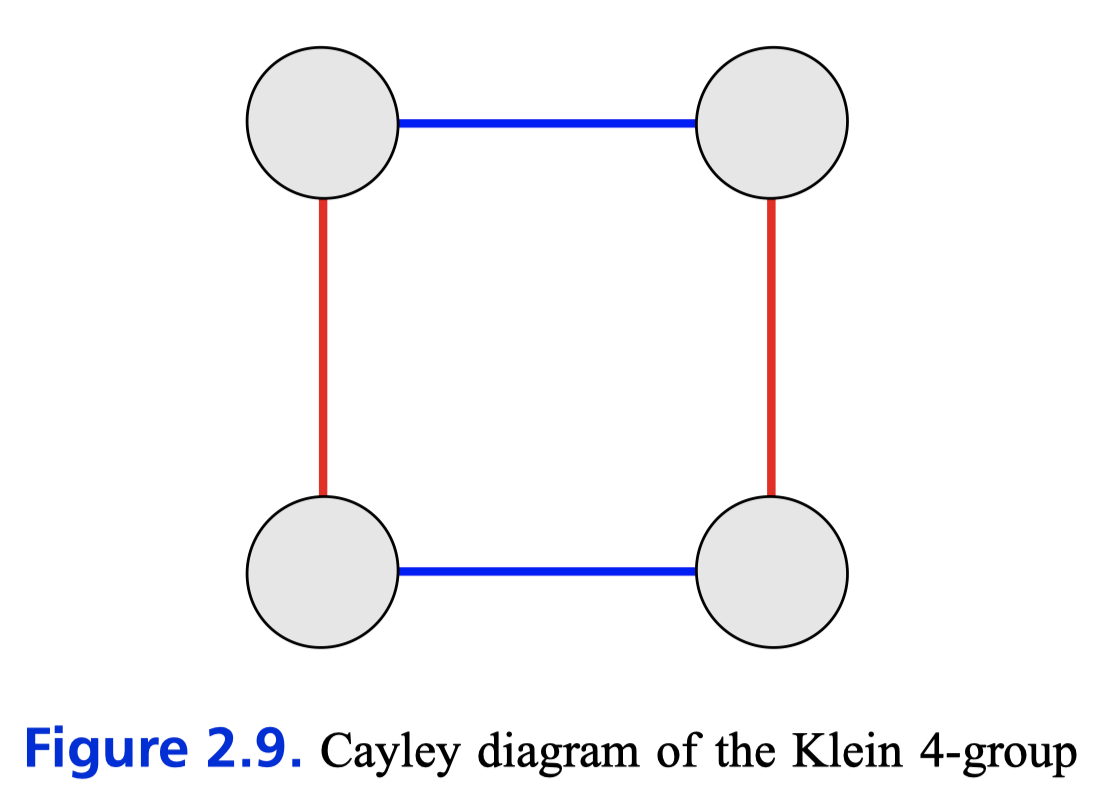
\includegraphics[width=.4\textwidth]{fig/Group/Cayley-Klein-4.png}
\end{figure}

凯利图包含如下要素:
\begin{enumerate}
\setlength{\itemsep}{0pt}
\setlength{\parsep}{0pt}
\setlength{\parskip}{0pt}
    \item 节点:代表群中的元;
    \item 有向边:不同颜色的边代表不同的“乘法”运算
\end{enumerate}

\begin{framed}
%\verb|\documentstyle[ifthen,12pt,titlepage]{article}|
\textcolor{red}{Cayley图的阅读方法:}

在观察 Cayley 图时,特别注意图中的\textbf{单位元}和从单位元出发的不同颜色的\textbf{边}。以下图的对称群$S_3$为例:
\begin{figure}[H]
    \centering
    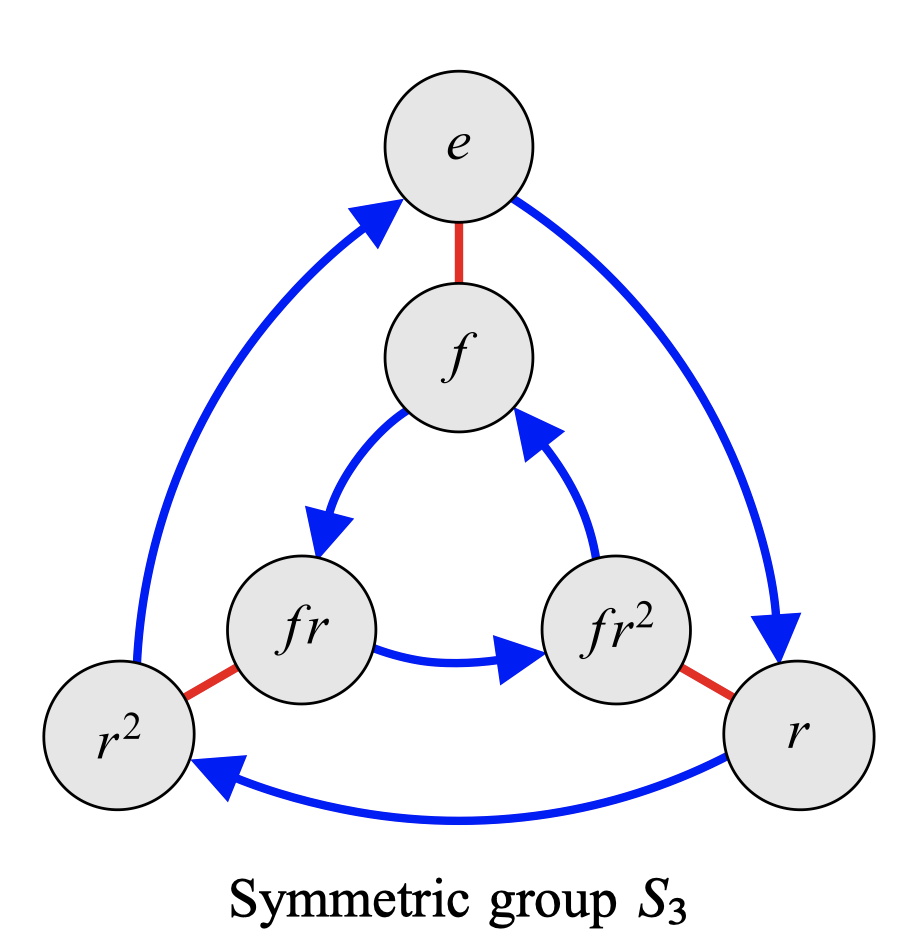
\includegraphics[width=.3\textwidth]{fig/Group/Cayley-S3.png}
\end{figure}

图中的单位元是$e$,从$e$出发的边有两种颜色:蓝色和红色;其中蓝色的边到达的节点是$r$,红色的边到达的节点是$f$;因此,这个群上定义了两种“乘法”运算,分别是:$e \cdot r = r,e \cdot f = f$。

进而可以推导出群上的其它运算:

$r \cdot r = r^2, \ r^2 \cdot r = e$(蓝色边);

$e \cdot f = f, \ r \cdot f = fr^2, \ fr^2 \cdot f = r, \ r^2 \cdot f = fr, \ fr \cdot r = r^2$(红色边);

$f \cdot r = fr, \ fr \cdot r = fr^2, \ fr^2 \cdot r = f$($r$与$f$的组合运算)
\end{framed}

\subsubsection{轨道(orbits)}
\begin{figure}[H]
    \centering
    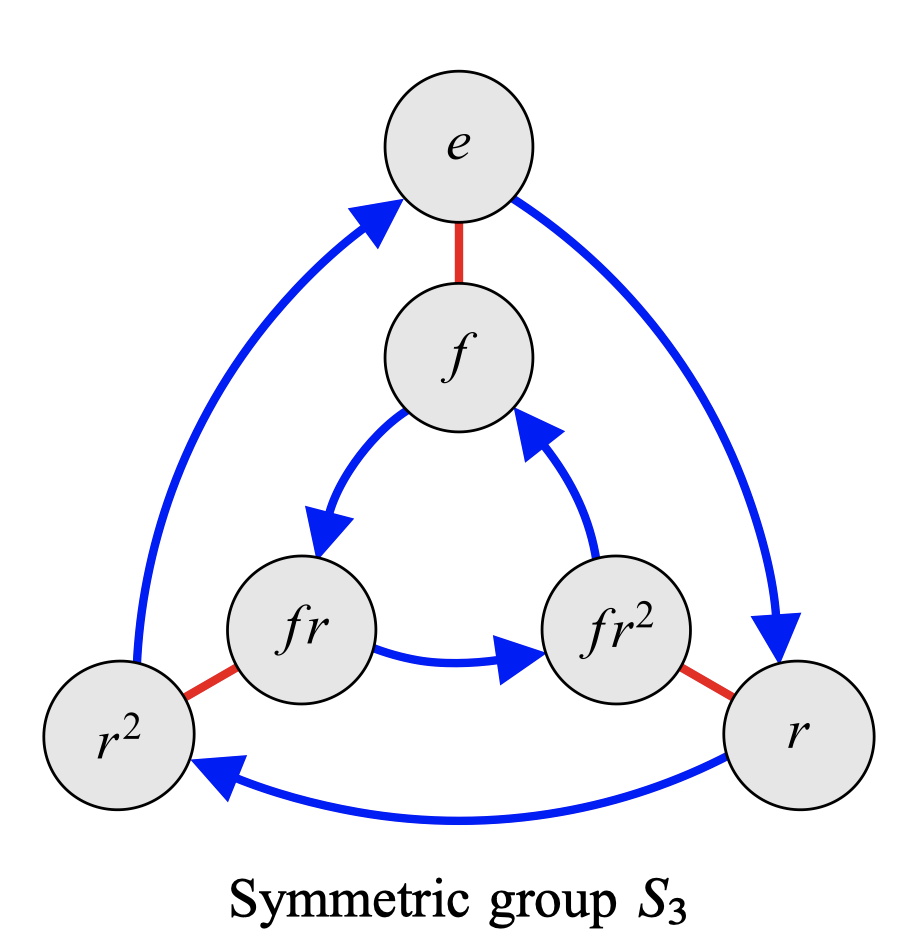
\includegraphics[width=.3\textwidth]{fig/Group/Cayley-S3.png}
\end{figure}
观察上图的对称群$S_3$,从单位元$e$出发,沿蓝色箭头指向,可以得到循环群$C_3$。这个循环叫做元素$r$的轨道(Starting at the identity $e$, the blue arrows lead in a cycle around the outside of the diagram, tracing out a copy of $C_3$ inside $S_3$. The standard term for this cycle is the \textbf{orbit} of the element $r$)。\textbf{群中的每个元素都有对应的轨道}。

轨道通常用它经过的元素集合来表示,例如$\{e, r, r^2\}$,$\{e, f\}$。

计算元素$fr^2$轨道的方法:进行一次$f$运算,然后进行两次$r$运算,依次进行;这样,可以得到$fr^2$的轨道为\{$e, fr^2\}$。

\subsection{循环图(Cycle Graph)}
因为每个轨道都是一个循环,这些轨道可以构成一个图,叫做循环图。例如,$S_3$的循环图如下图所示:
\begin{figure}[H]
    \centering
    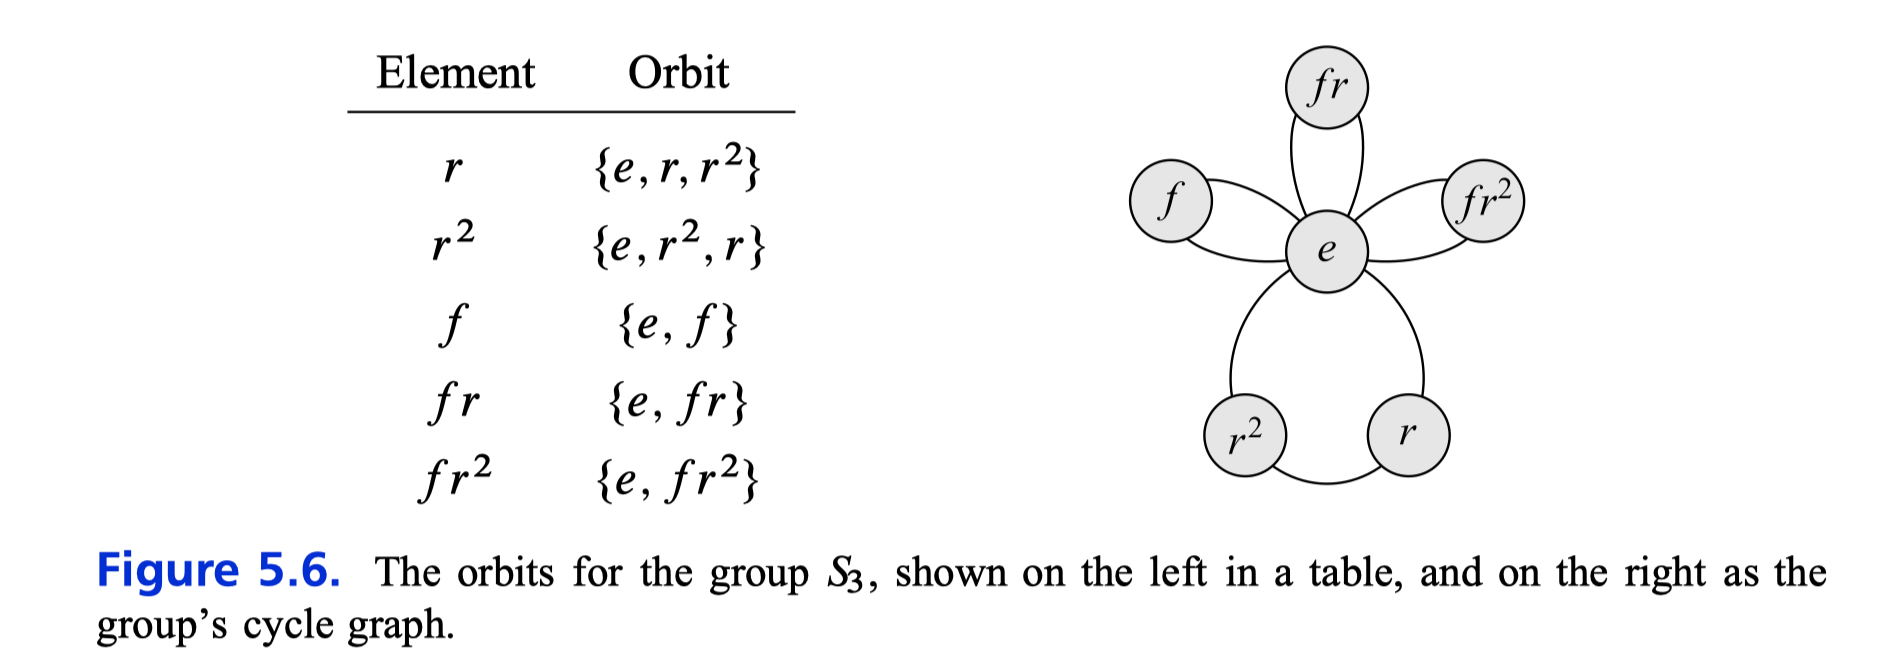
\includegraphics[width=.8\textwidth]{fig/Group/CycleGraph-S3.png}
\end{figure}

循环群的Cycle Graph和 Cayley Diagrams 看起来是基本一样的,因为循环群中只有一个循环。区别仅在于Cycle Graph中的边一般没有箭头。
\begin{figure}[H]
    \centering
    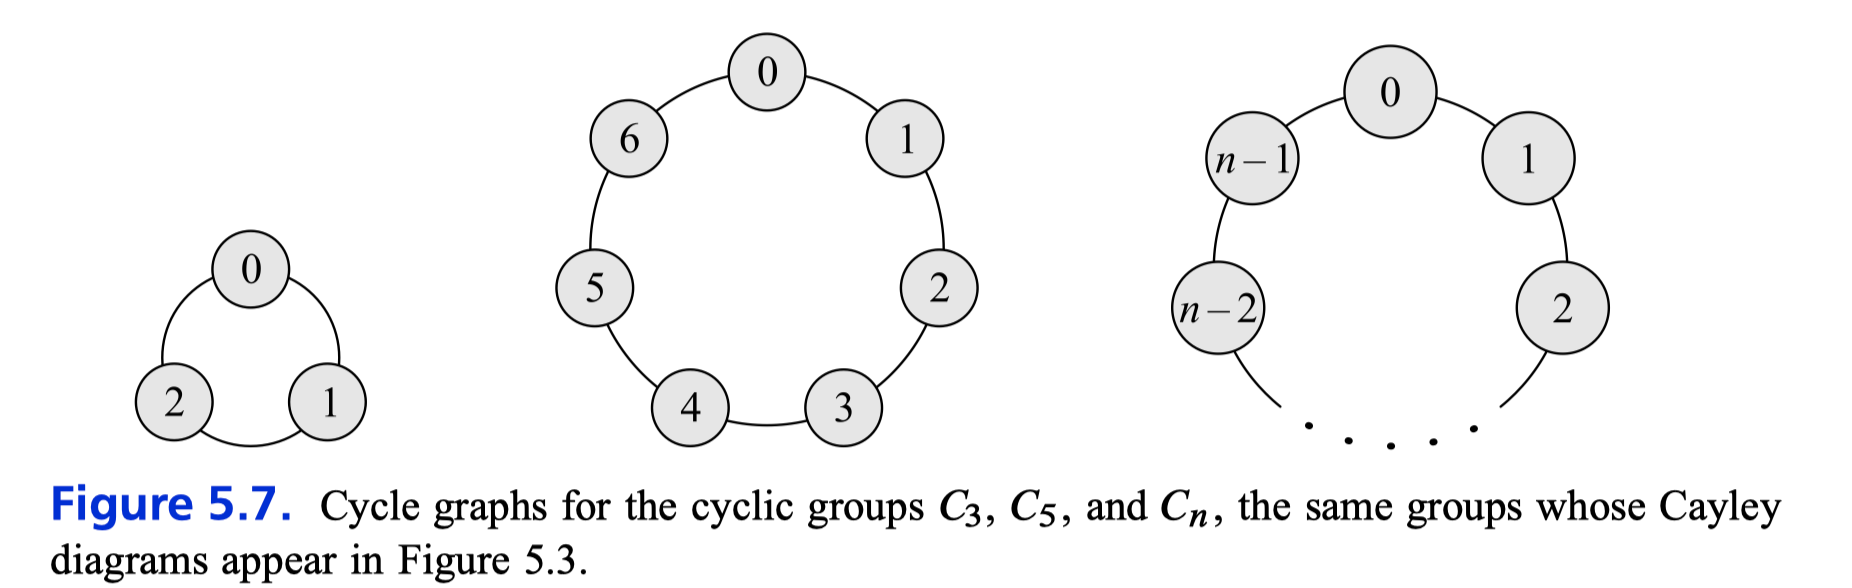
\includegraphics[width=.8\textwidth]{fig/Group/CycleGraph-CyclicGroup.png}
\end{figure}

\subsection{乘法表(Multiplication Table)}
\begin{figure}[H]
    \centering
    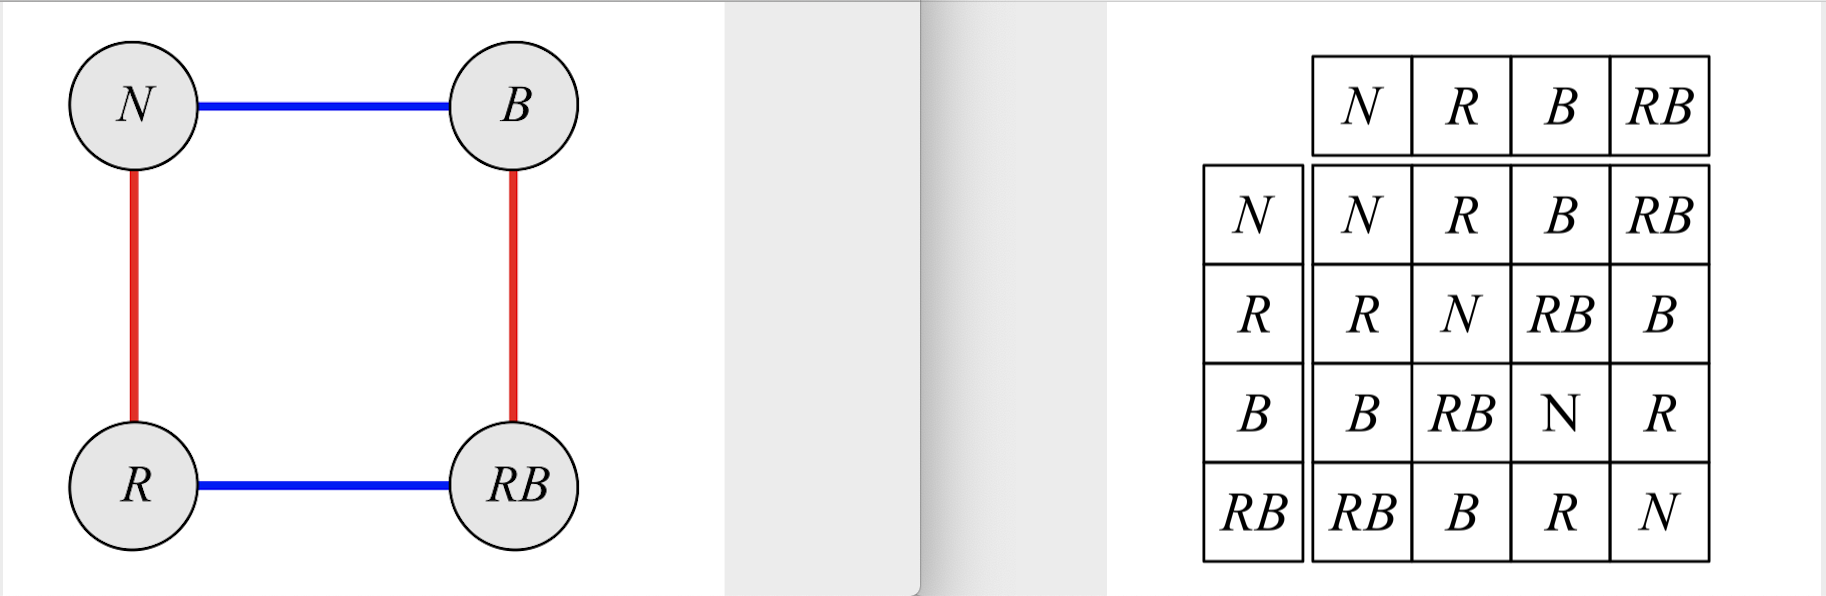
\includegraphics[width=.7\textwidth]{fig/Group/MultiplicationTable_Klein4.png}
     \caption{Cayley 图和 Multiplicaiton Table 的对应关系}
\end{figure}

\section{常见的群}
\subsection{反演群$V_n$(Klein n-group)}
想象一下墙上有两个开关,每个开关都有2种开关状态;一共有$2^2 = 4$中状态,构成的群是反演群$V_4$。

反演群的Cayley图如下:
\begin{figure}[H]
    \centering
    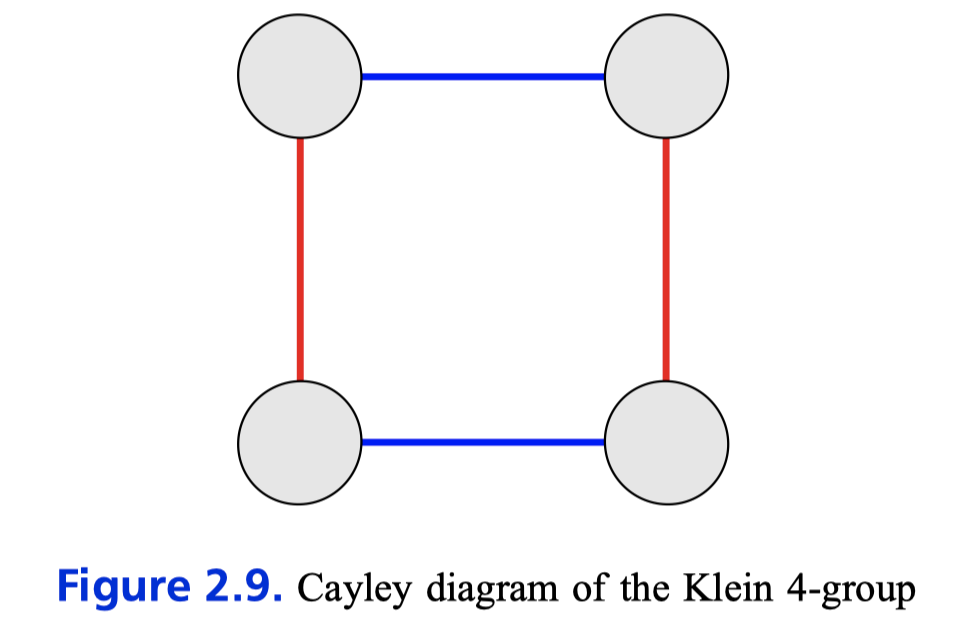
\includegraphics[width=.5\textwidth]{fig/Group/Cayley-V4.png}
\end{figure}

\subsection{循环群$C_n$(Cyclic Group)}
\textbf{循环群描述了物体的旋转对称性(rotational symmetry)}。

循环群的Cayley 图和乘法表如下图所示:
\begin{figure}[H]
    \centering
    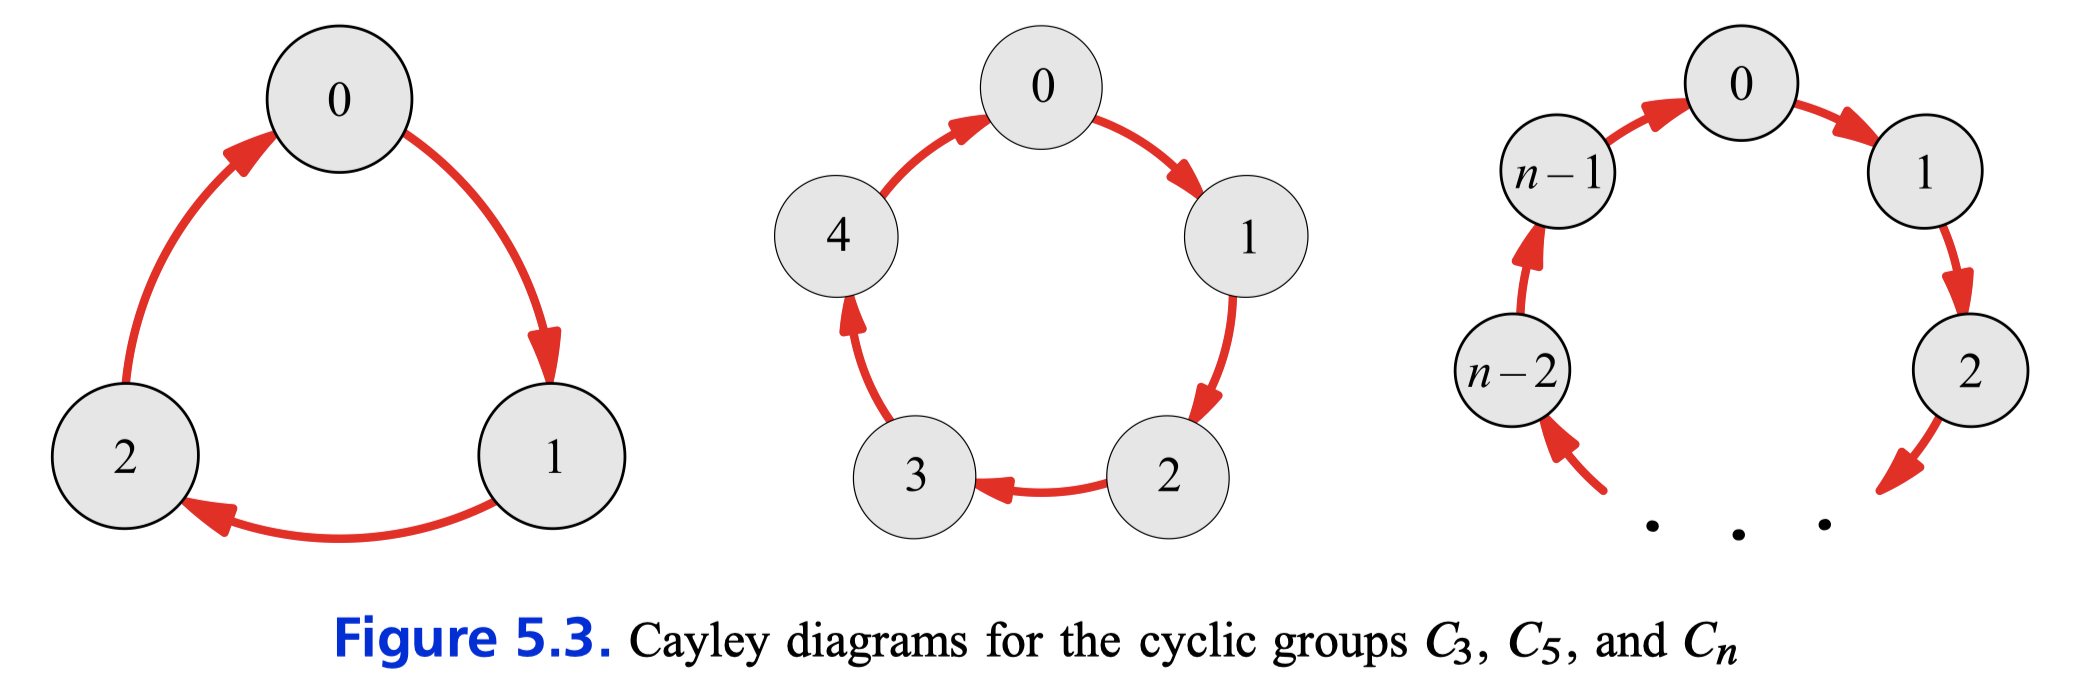
\includegraphics[width=1\textwidth]{fig/Group/Cayley-Cyclic-Group-Examples.png}
\end{figure}
\begin{figure}[H]
    \centering
    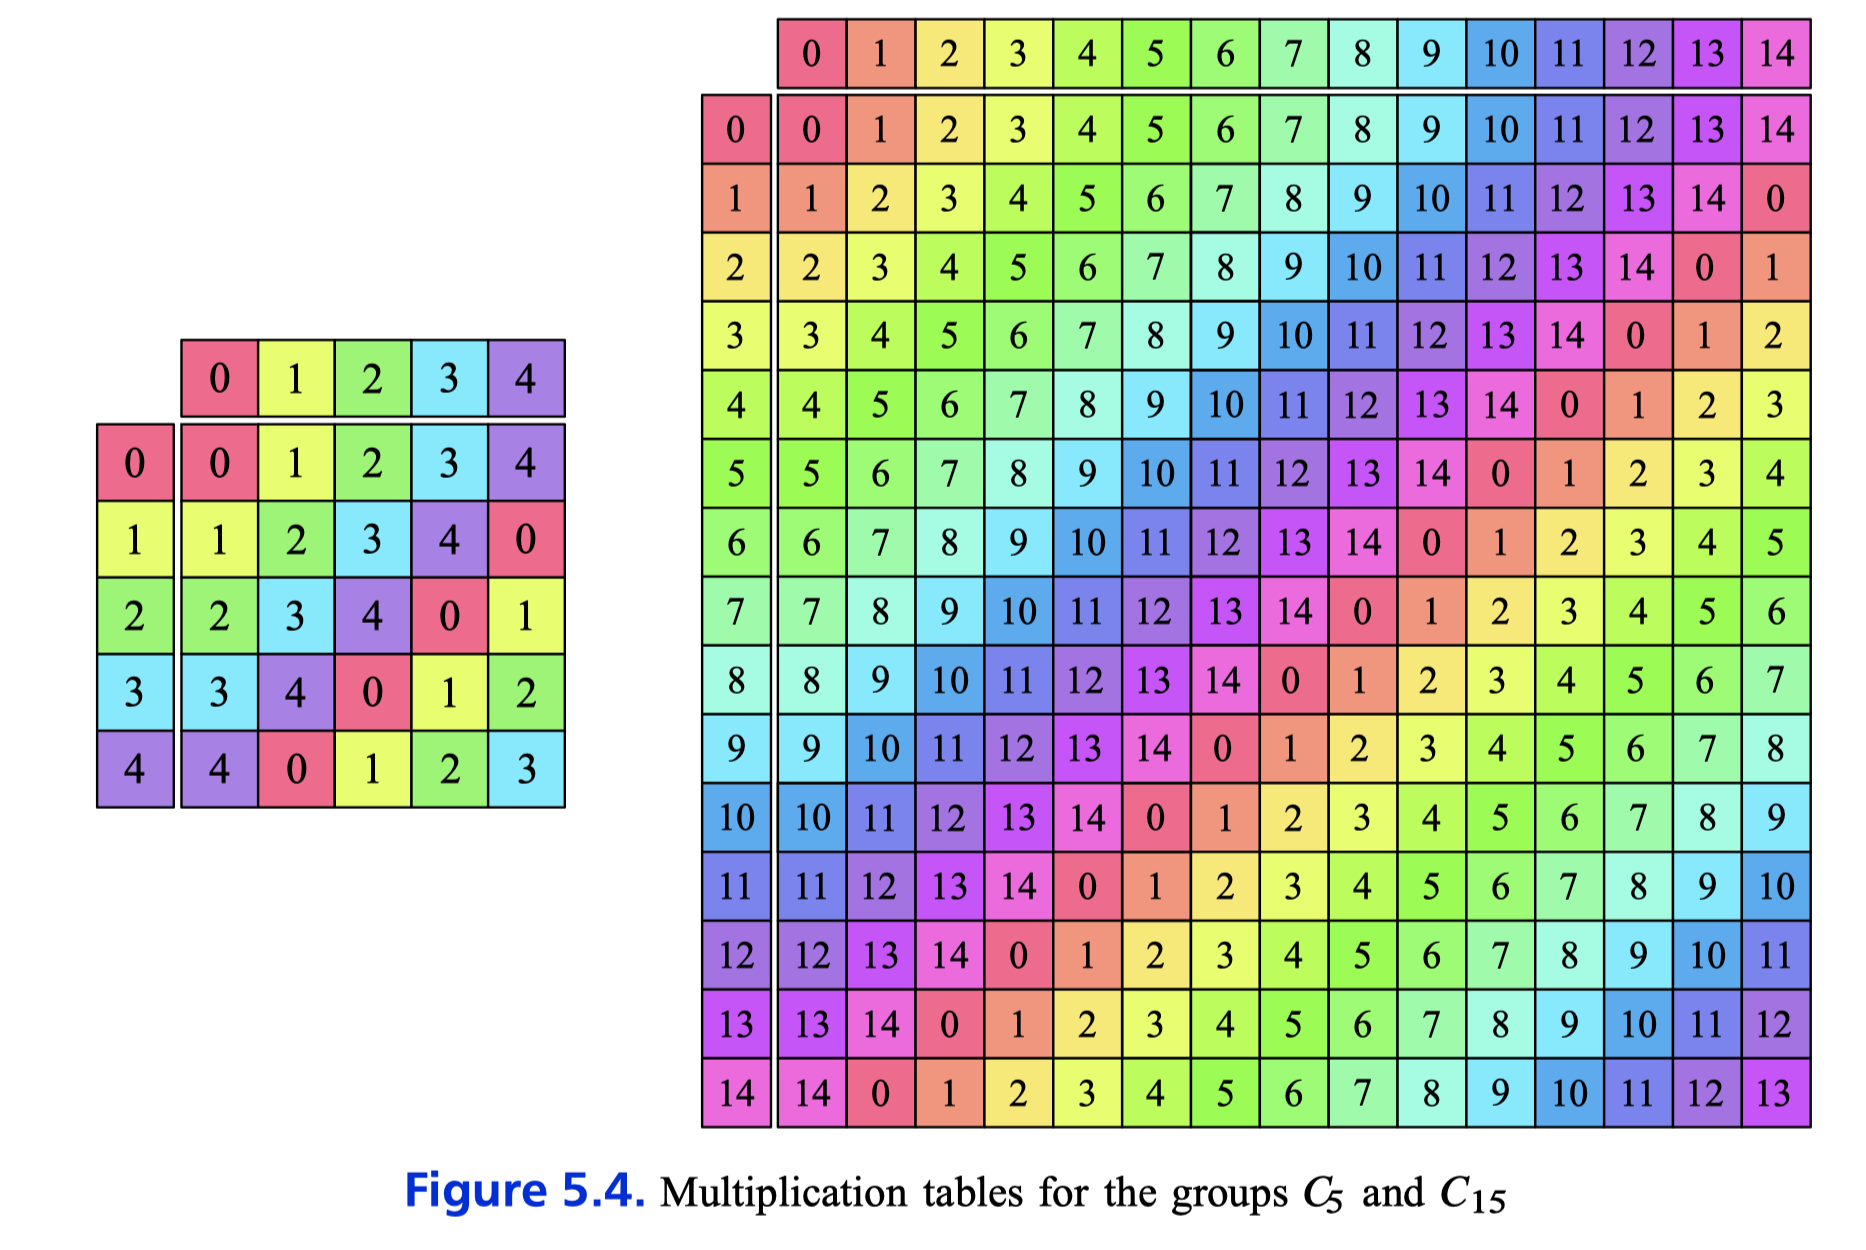
\includegraphics[width=.8\textwidth]{fig/Group/MultiplicationTable_C5_C15.png}
\end{figure}

循环群$C_n$也可以表示为$\mathbb{Z}_n$。这是因为把$C_n$可以看做包含了前$n$个非负元素的整数集合。

通过对5进行\textbf{模加运算},可以得到循环群$C_5$。

\subsection{阿贝尔群(Abelian Group)}
阿贝尔群是满足\textbf{交换律}的群。

\textbf{所有的循环群都是阿贝尔群}

\subsubsection{是否满足交换律在 Cayley 图上的区别}
是否满足交换律的群在 Cayley 图上有明显区别。如下图所示,红色代表运算$a$,蓝色代表运算$b$;先红色再蓝色代表$ab$,先蓝色再红色代表$ba$;如果不满足交换律(左图),即$ab\neq ba$,那么两条路径不会相交;反之会相交(右图):
\begin{figure}[H]
    \centering
    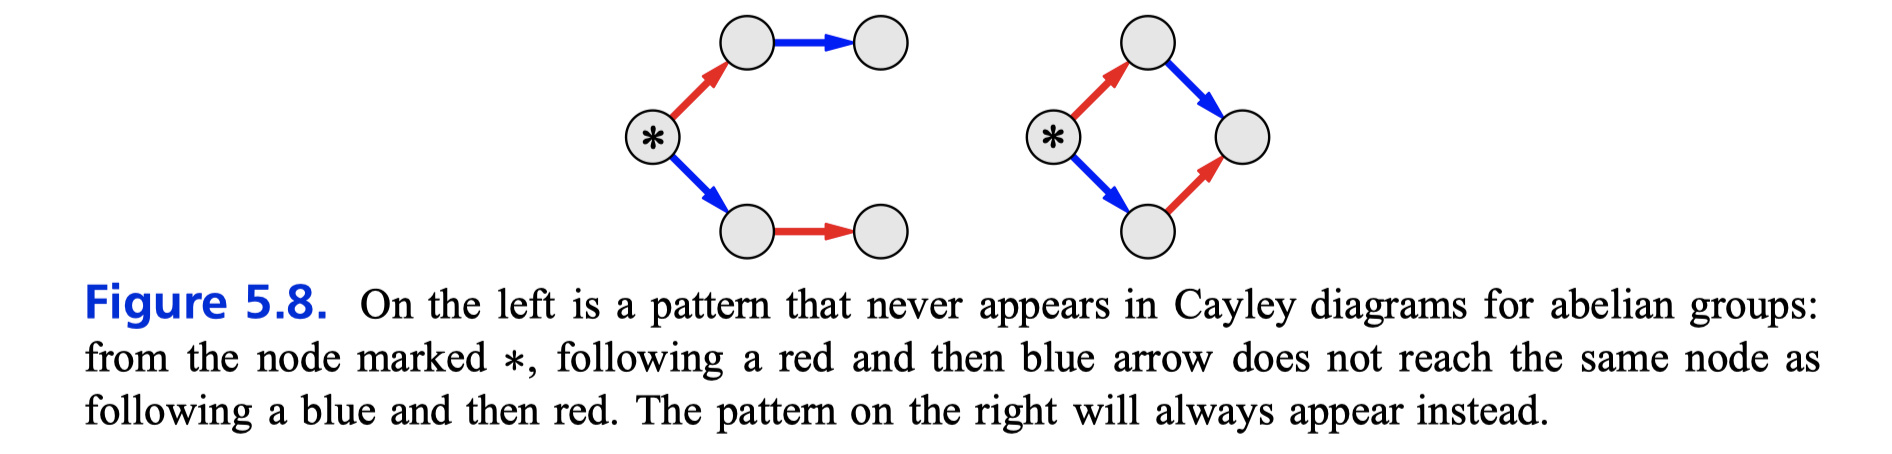
\includegraphics[width=1\textwidth]{fig/Group/Cayley-Noncommutativity.png}
\end{figure}

\subsubsection{是否满足交换律在乘法表上的区别}
如果满足交换律,有:$ab=ba$,那么所以,乘法表上的对应元素是关于对角线对称的,如下图:
\begin{figure}[H]
    \centering
    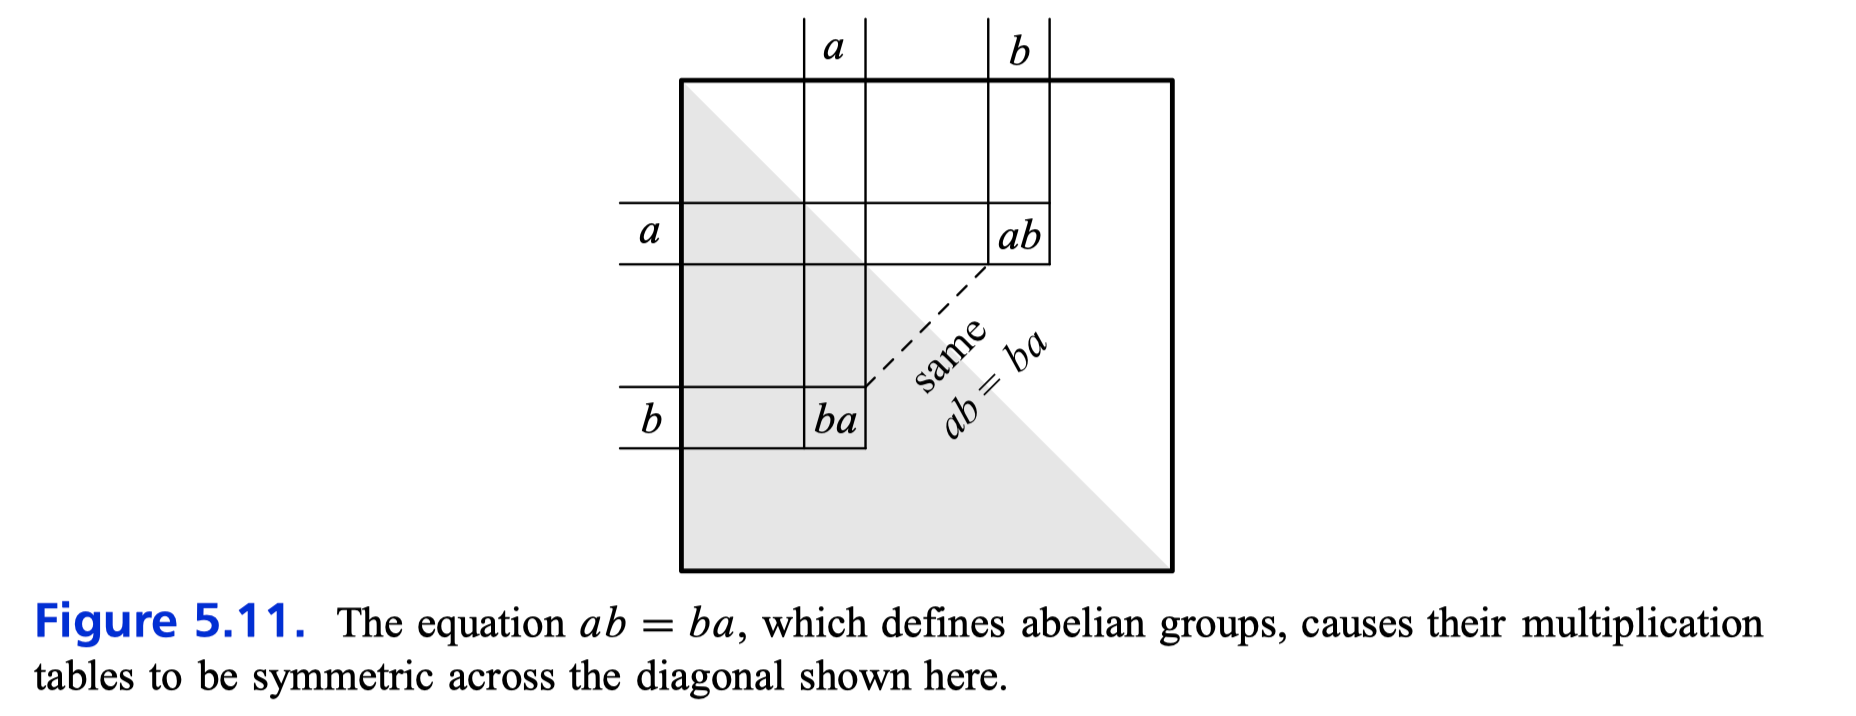
\includegraphics[width=1\textwidth]{fig/Group/MultiplicationTable-Commutativity.png}
\end{figure}

阿贝尔群的 Cycle Graph 如下图所示:
\begin{figure}[H]
    \centering
    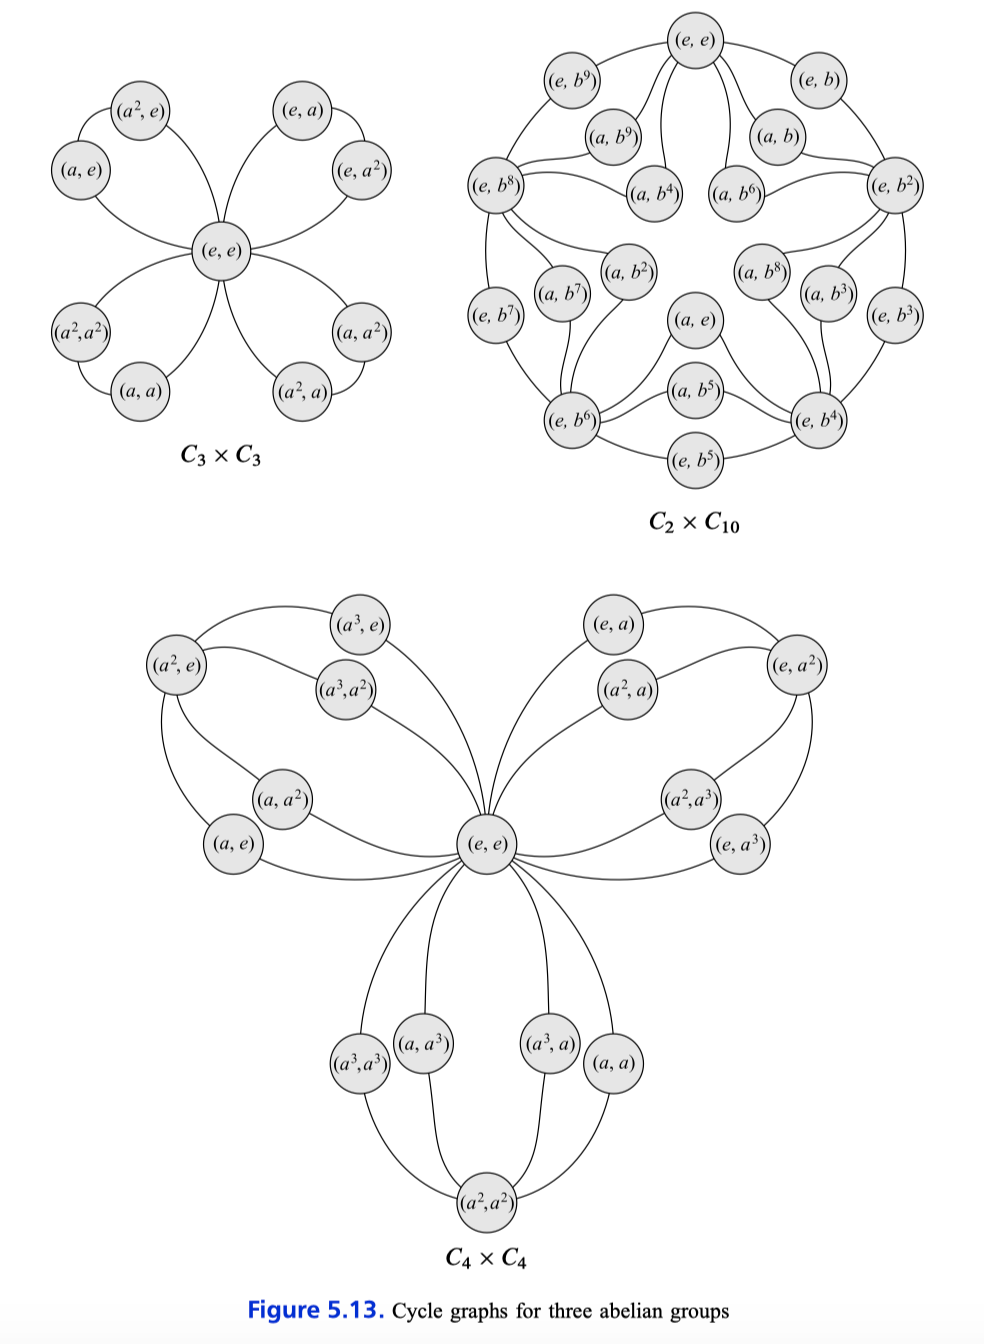
\includegraphics[width=.5\textwidth]{fig/Group/CycleGraph-Abelian.png}
\end{figure}

\subsection{二面体群(dihedral group)}
\textbf{二面体群不止描述旋转对称性(rotational symmetry),还描述了\textbf{左右对称性(bilateral symmetry)}}。

二面体群描述了正$n$边形的对称性,表示为$D_n$。循环群$C_n$的所有运算,也都是$D_n$的运算,因为$D_n$描述了旋转对称性;同时,因为$D_n$还描述了左右对称性,所以$D_n$包含的元素个数比$C_n$多。$C_n$包含$n$个元,$D_n$包含$2n$个元。

二面体群的Cayley 图和乘法表如下图所示:
\begin{figure}[H]
    \centering
    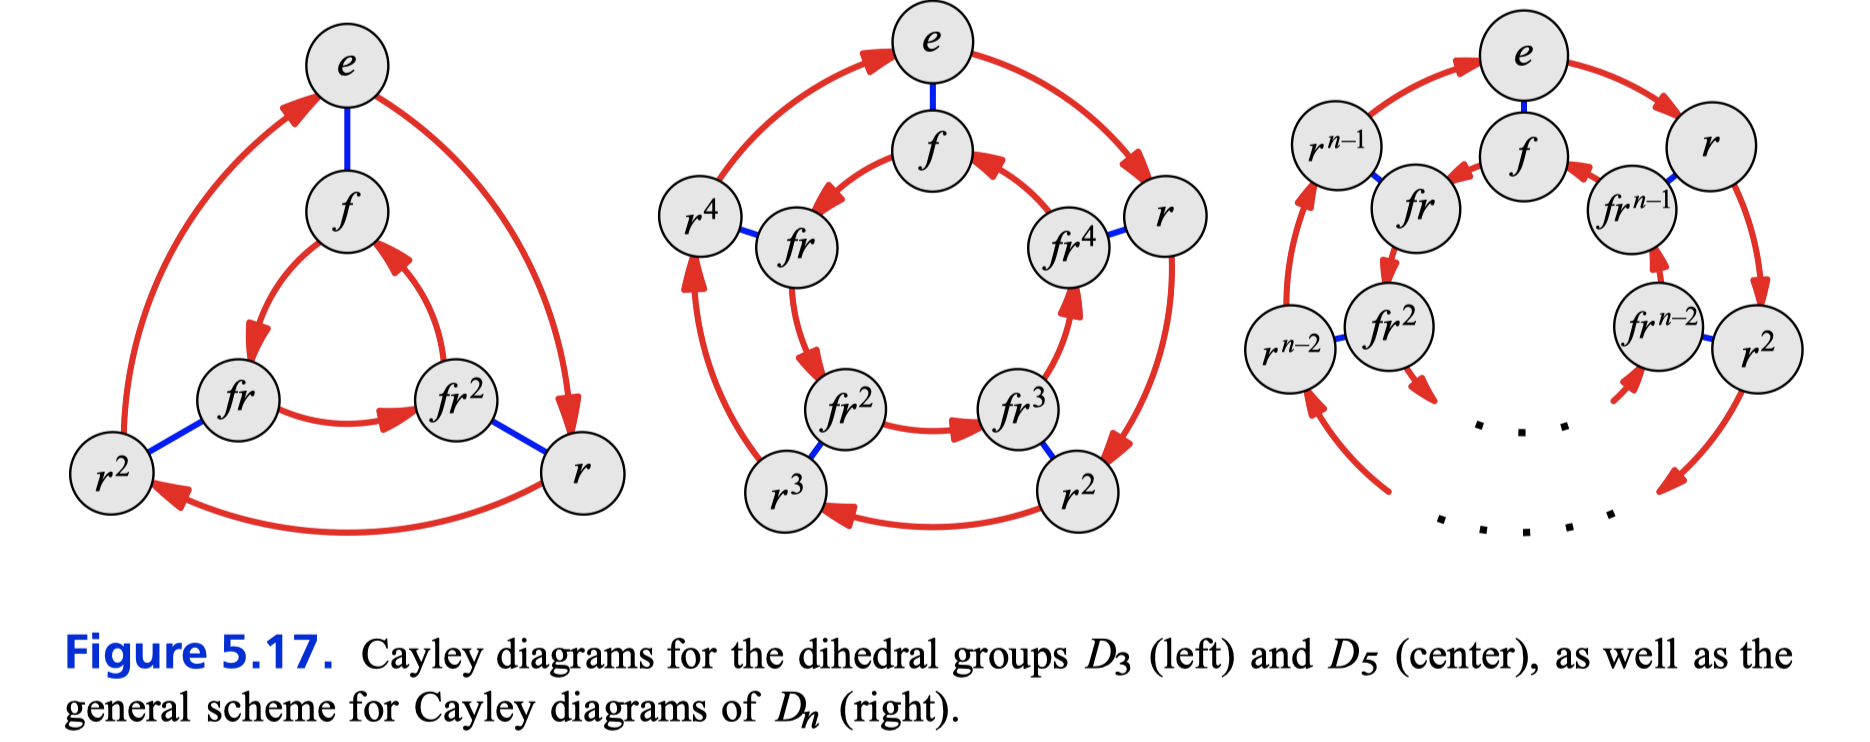
\includegraphics[width=1\textwidth]{fig/Group/Cayley-Dihedral-Group-Examples.png}
\end{figure}
\begin{figure}[H]
    \centering
    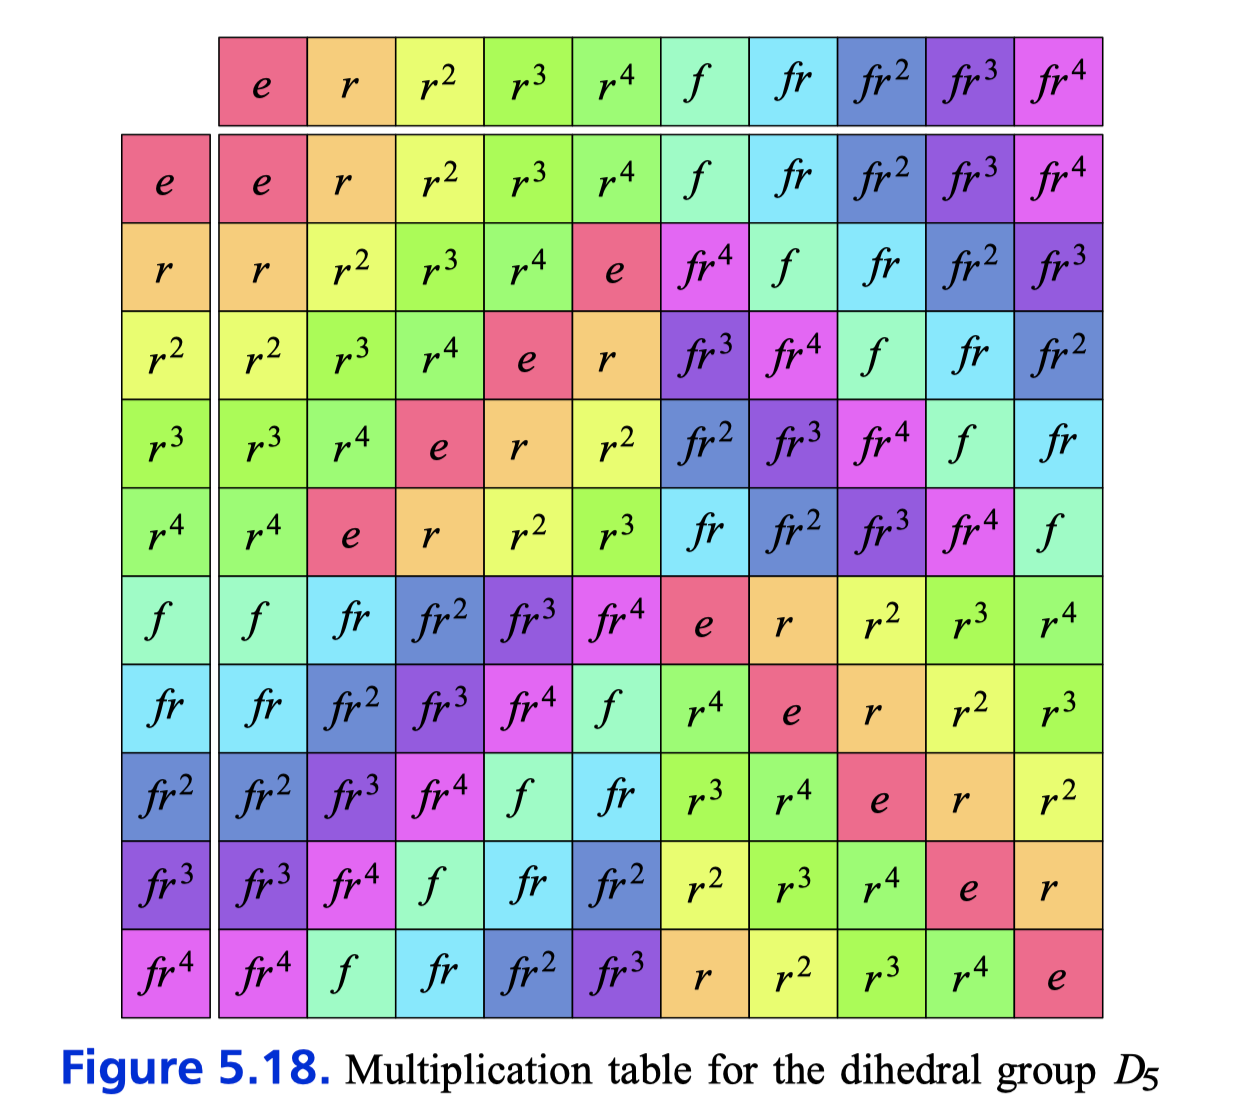
\includegraphics[width=.8\textwidth]{fig/Group/MultiplicationTable-Dihedral-Group.png}
\end{figure}

观察$D_3$的Cayley图可以看出:外面的红圈是$r$的轨道,与$C_3$同构;里面的红圈是与外圈反向,是$C_3$的左陪集$fC_3$(待确认,应该没问题);

观察$D_5$的乘法表,可以很容易的将它按水平和竖直方向分成四个子块,得到一个$2\times 2$的乘法表:
\begin{figure}[H]
    \centering
    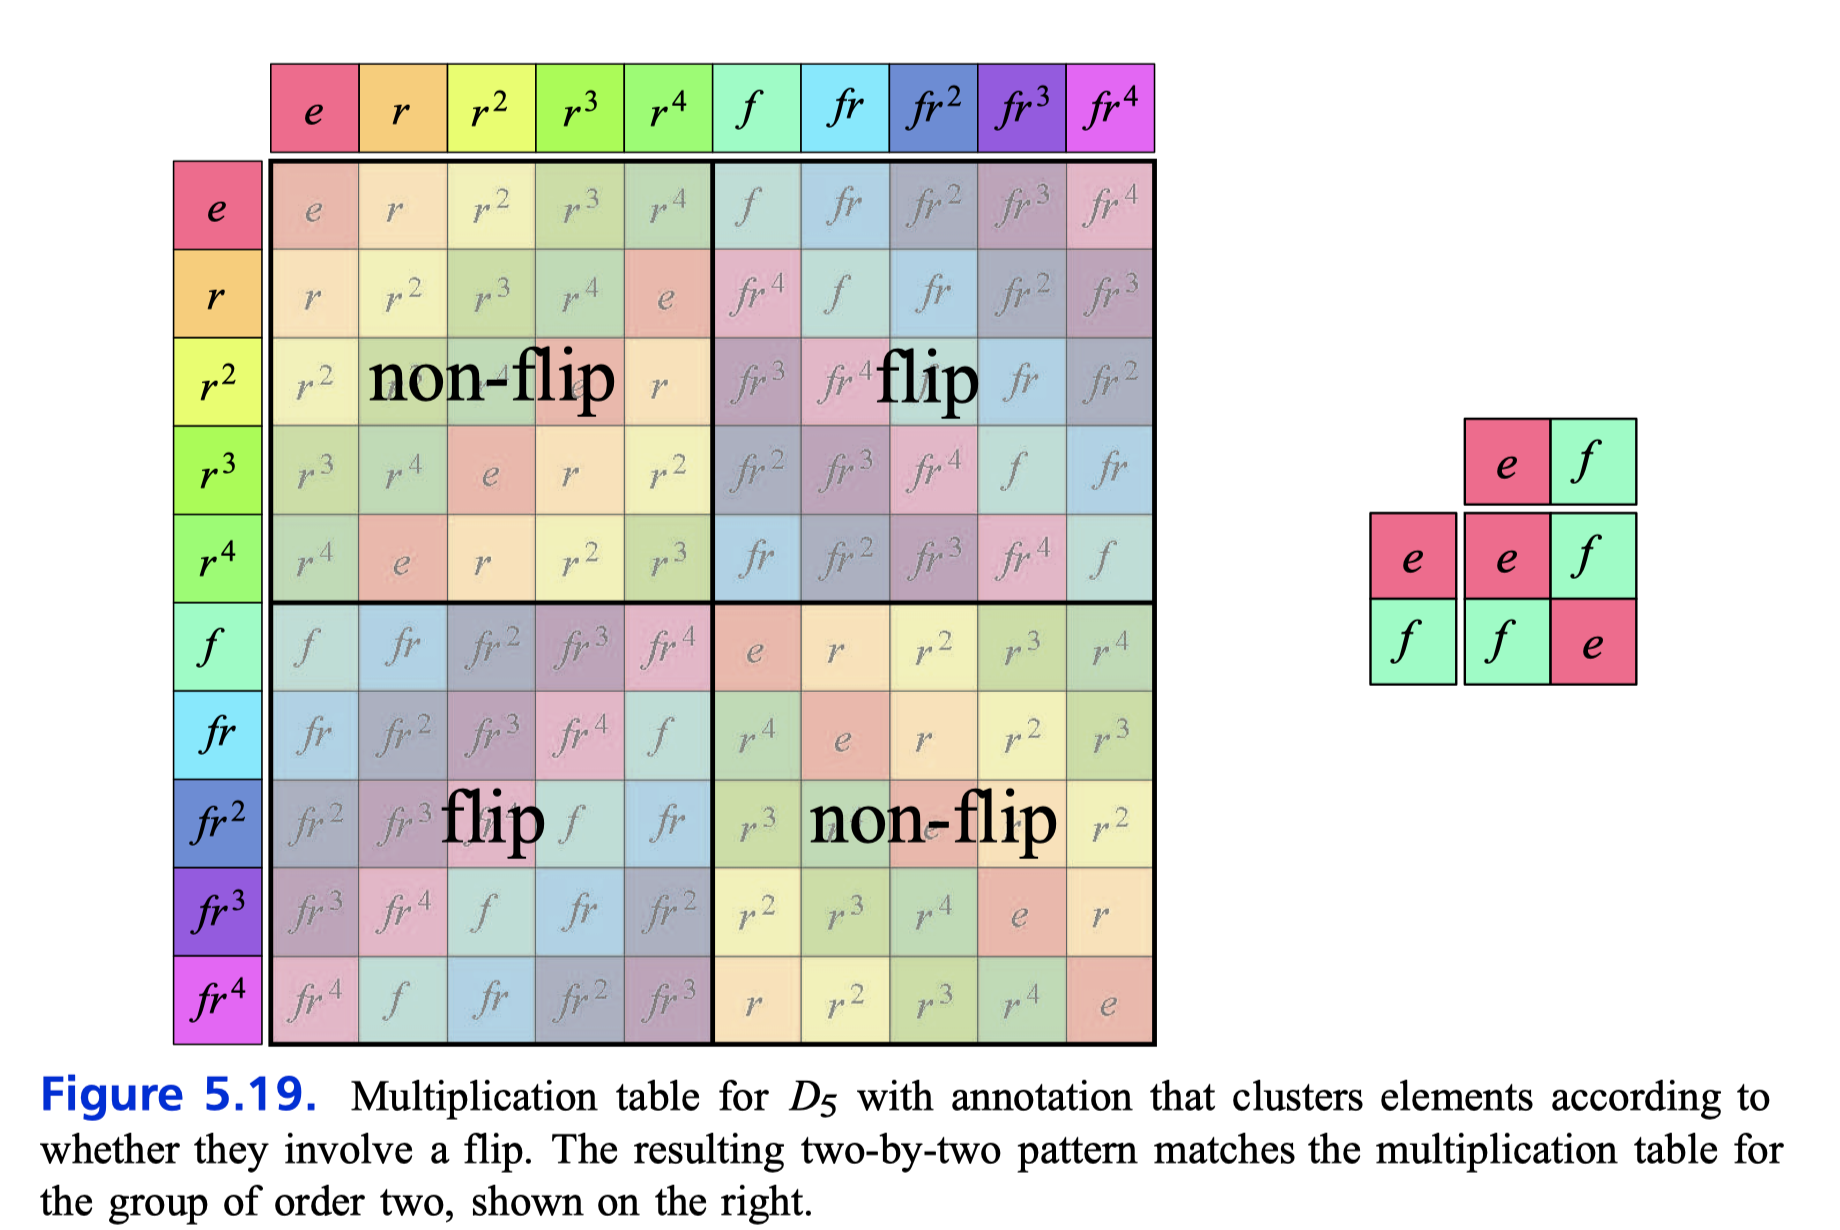
\includegraphics[width=1\textwidth]{fig/Group/MultiplicationTable-D5.png}
\end{figure}
\textcolor{red}{这种划分方式揭示了$D_5$群的子结构;按照这种方式,对群进行划分,叫做取商(quotient);对$C_n$和$C_2$作半直积(semidirect product)可以得到$D_n$}

二面体群的Cycle Graph如下图所示:
\begin{figure}[H]
    \centering
    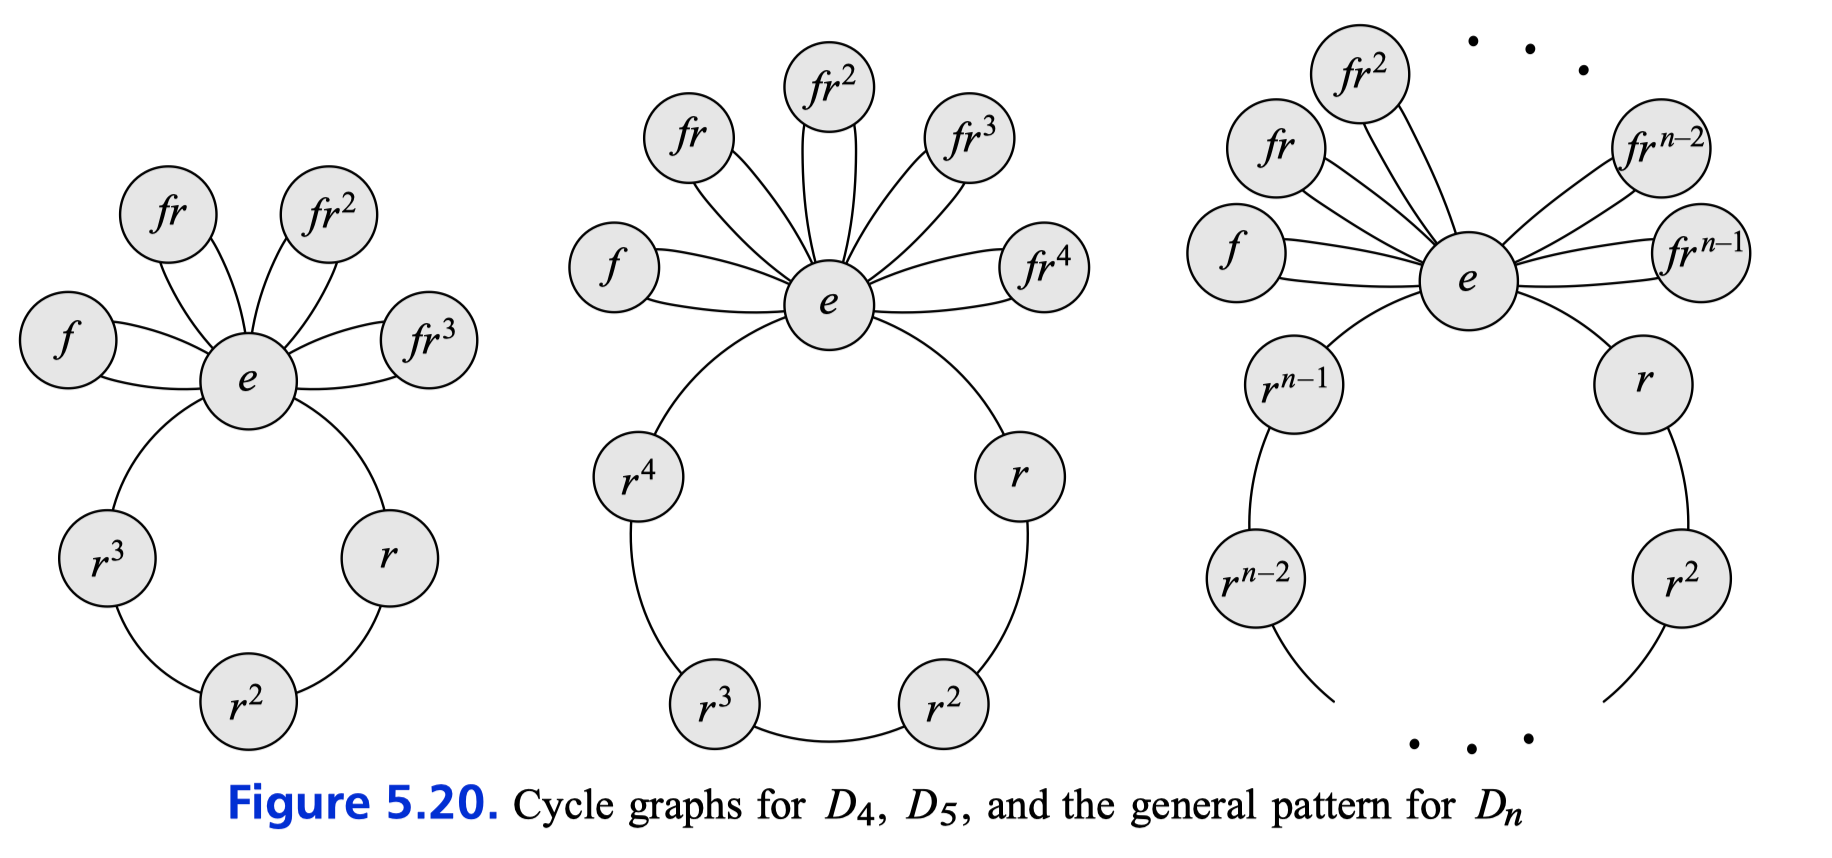
\includegraphics[width=1\textwidth]{fig/Group/CycleGraph-Dihedral.png}
\end{figure}

\subsection{对称群$S_n$}
对全体元素进行置换(permutation),构成的群,叫做对称群(The group of all permutations of a given size is called a symmetric group)。

对称群$S_n$包含有$n!$个元素,表示对$n$个元素进行全排列。

对称群的Cayley图如下:
\begin{figure}[H]
    \centering
    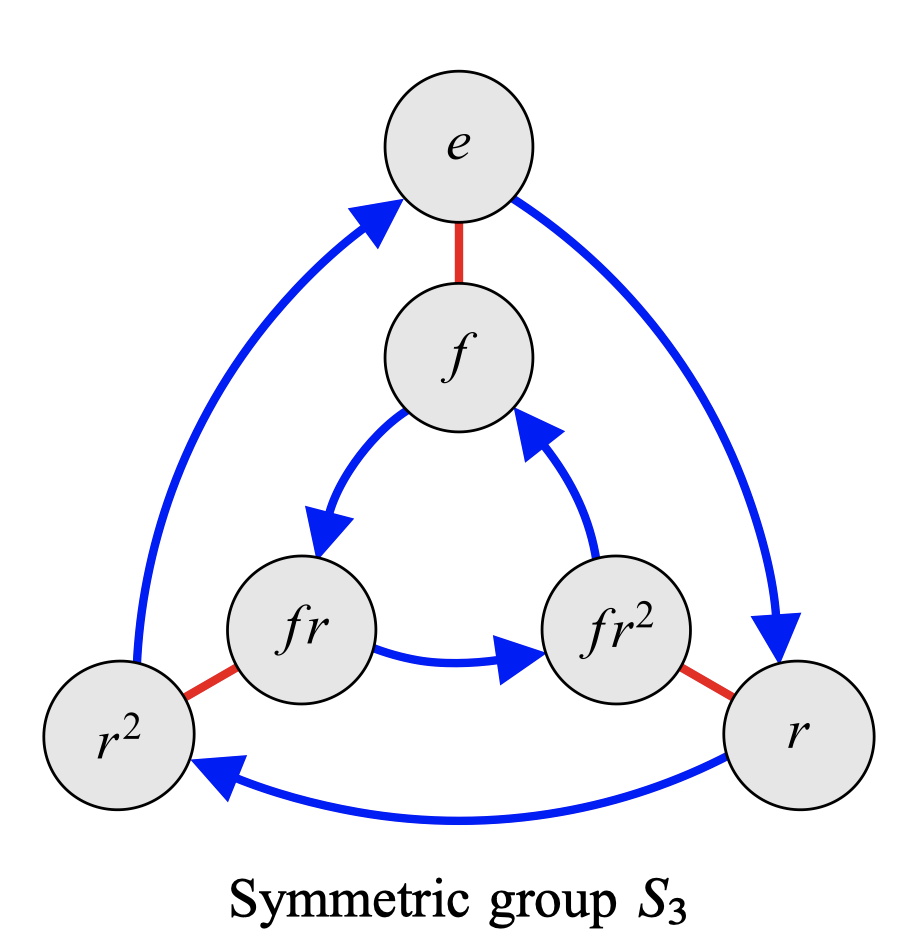
\includegraphics[width=.3\textwidth]{fig/Group/Cayley-S3.png}
\end{figure}
\begin{figure}[H]
    \centering
    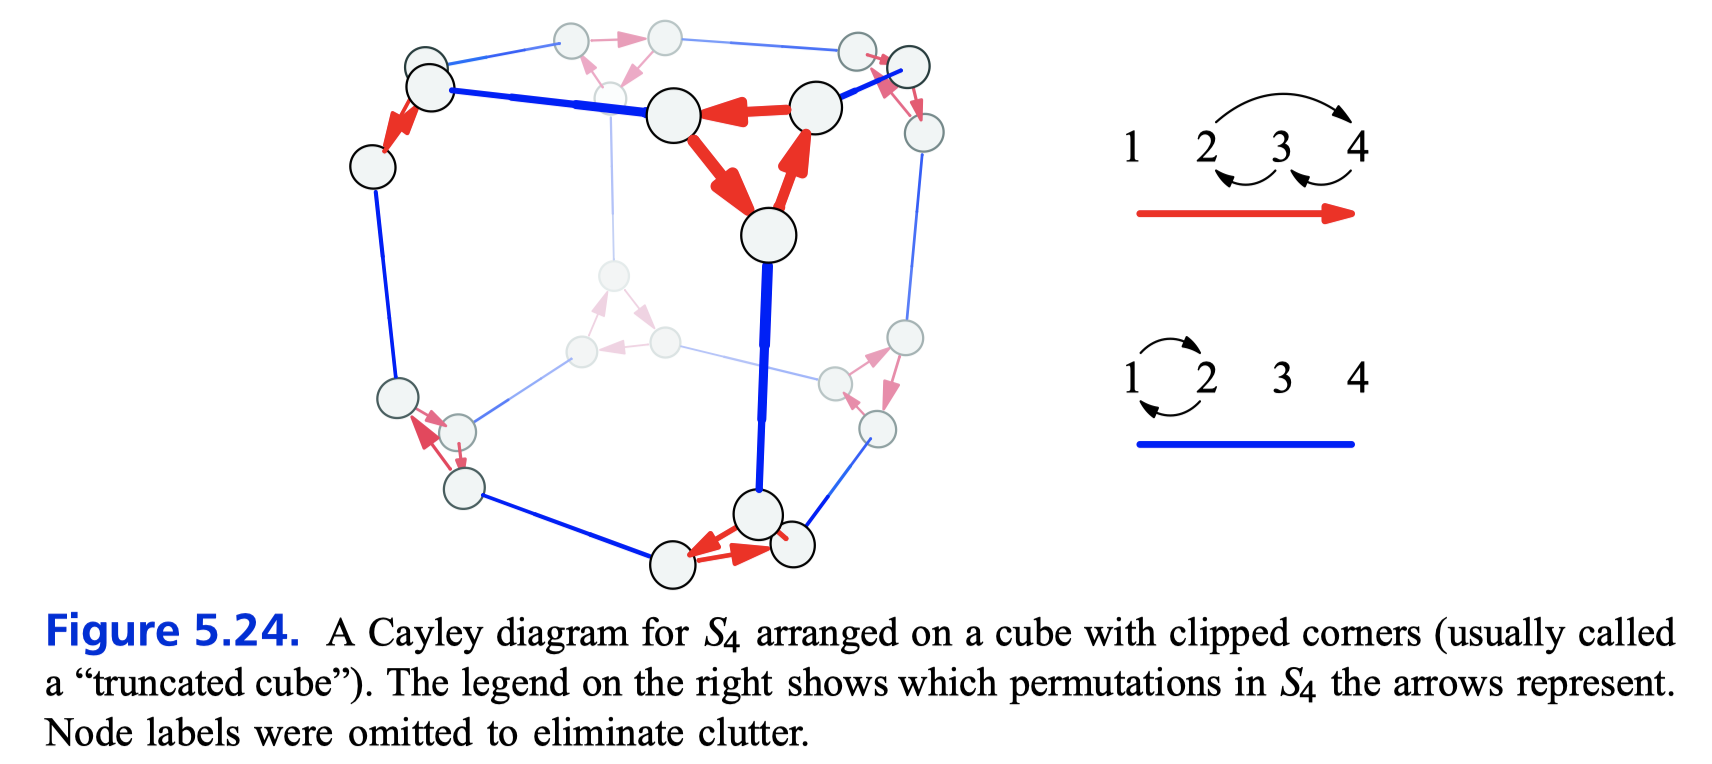
\includegraphics[width=1\textwidth]{fig/Group/Cayley-S4.png}
\end{figure}
\begin{figure}[H]
    \centering
    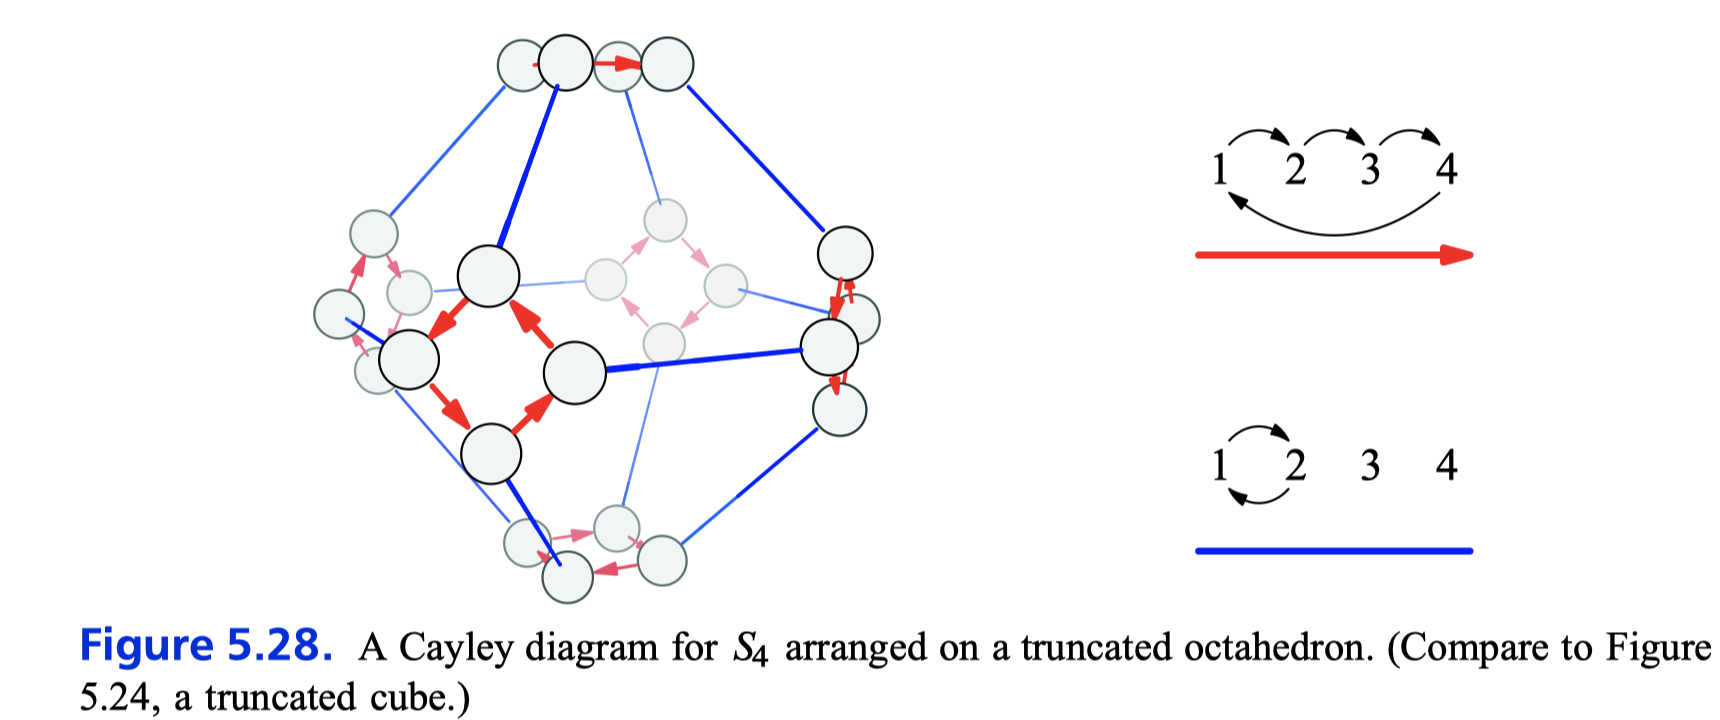
\includegraphics[width=1\textwidth]{fig/Group/Cayley-S4-Octahedron.png}
\end{figure}
从图中可以看出,$S_3$包含$3!=6$个元素,$S_4$包含$4!=24$个元素。

\subsection{交错群$A_n$}
对称群$S_n$包含$n!$个元素,交错群$A_n$包含其中$S_n$中一半的元素(Although the collection of all permutations of $n$ items forms a group, creating a group of permutations does not require taking all permutations of a given size. It is often possible to form a group from just some of the permutations from $S_n$. One famous way is to take exactly half of the elements of $S_n$, creating what is called an alternating group)。从$S_n$中随机挑选一半元素,很难构成群;一种可行的方法是对$S_n$中的每个元素进行“平方”运算,得到的集合刚好包含一半元素。举例如下:
\begin{figure}[H]
    \centering
    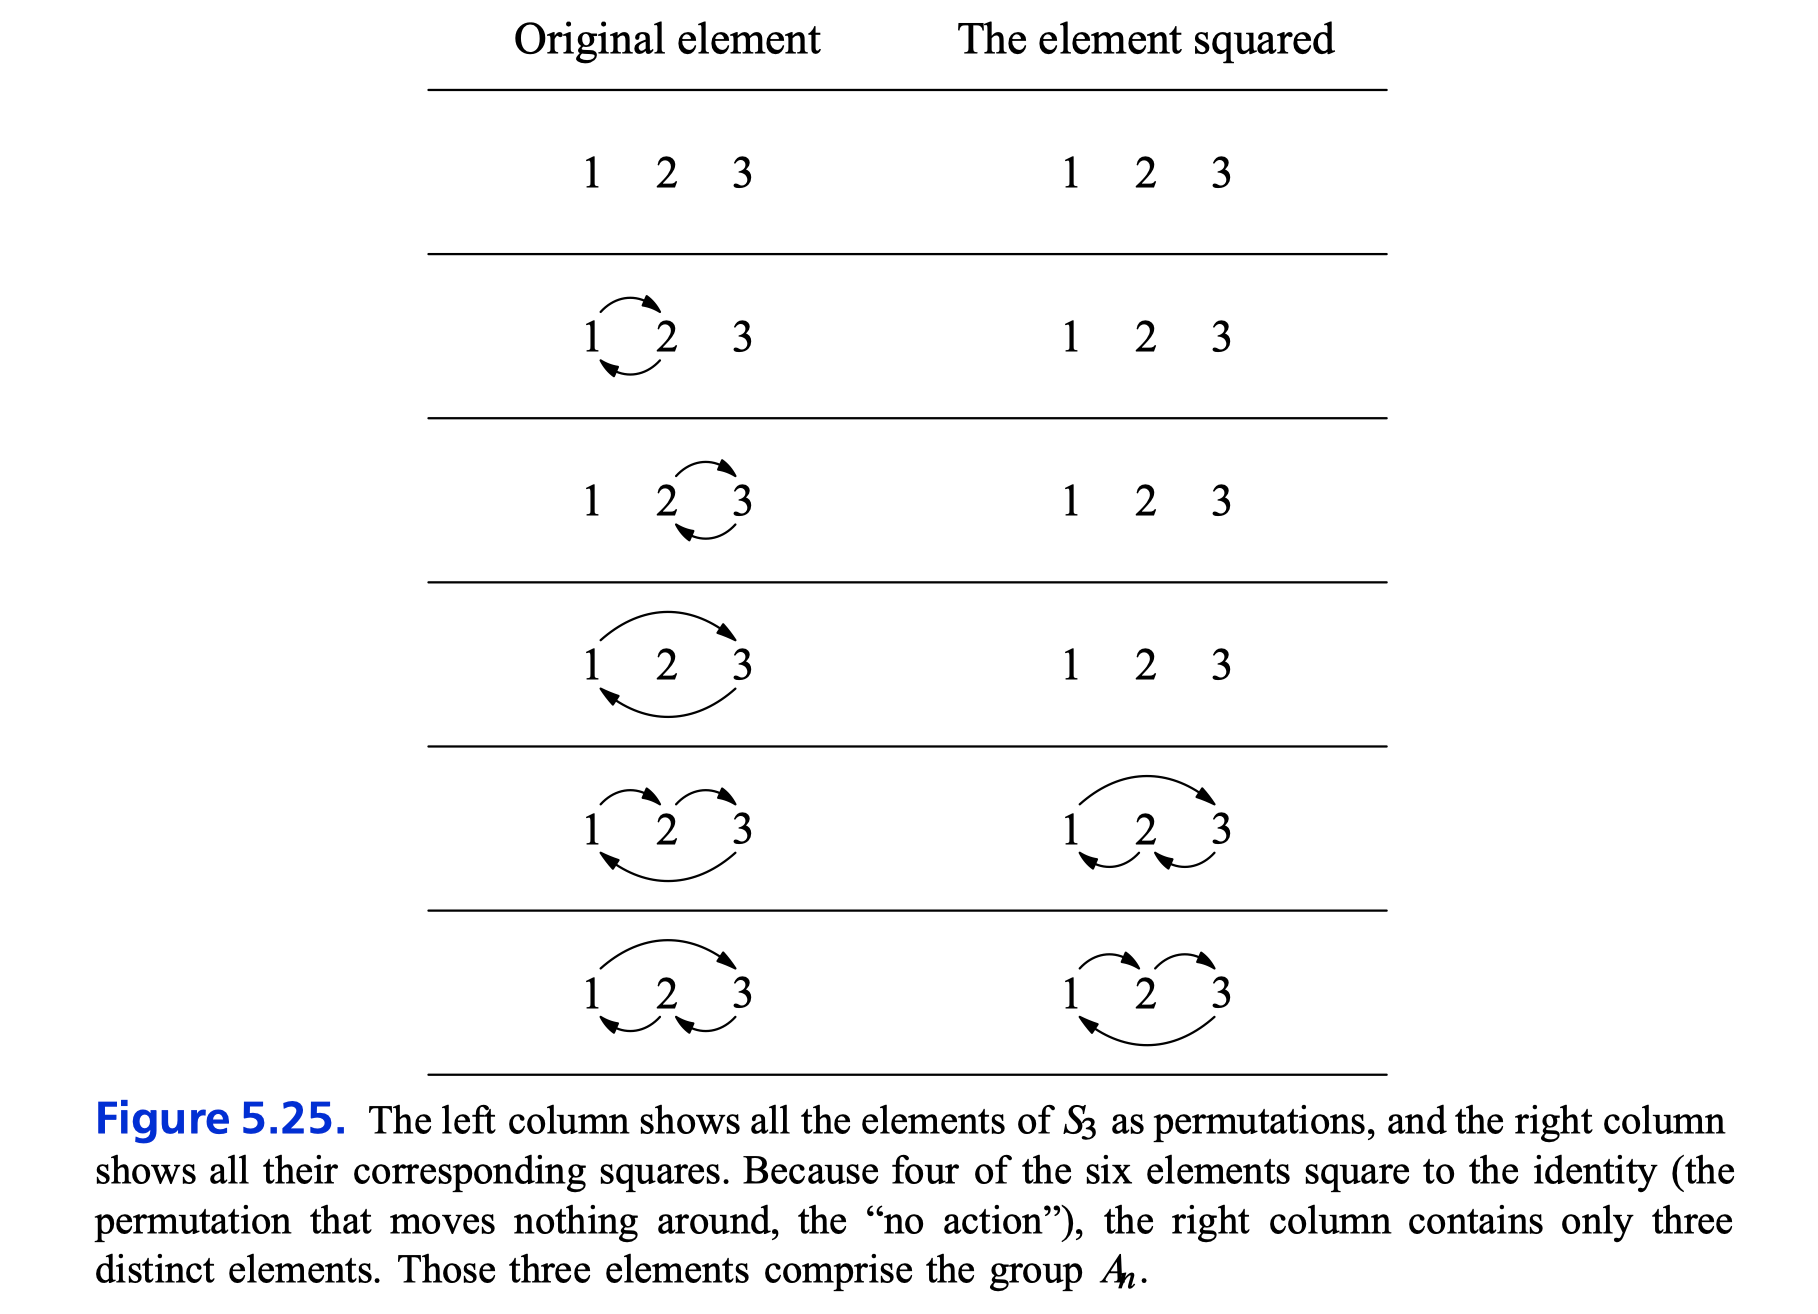
\includegraphics[width=1\textwidth]{fig/Group/AlternatingGroup-A3-creation.png}
\end{figure}

交错群的Cayley图如下:
\begin{figure}[H]
    \centering
    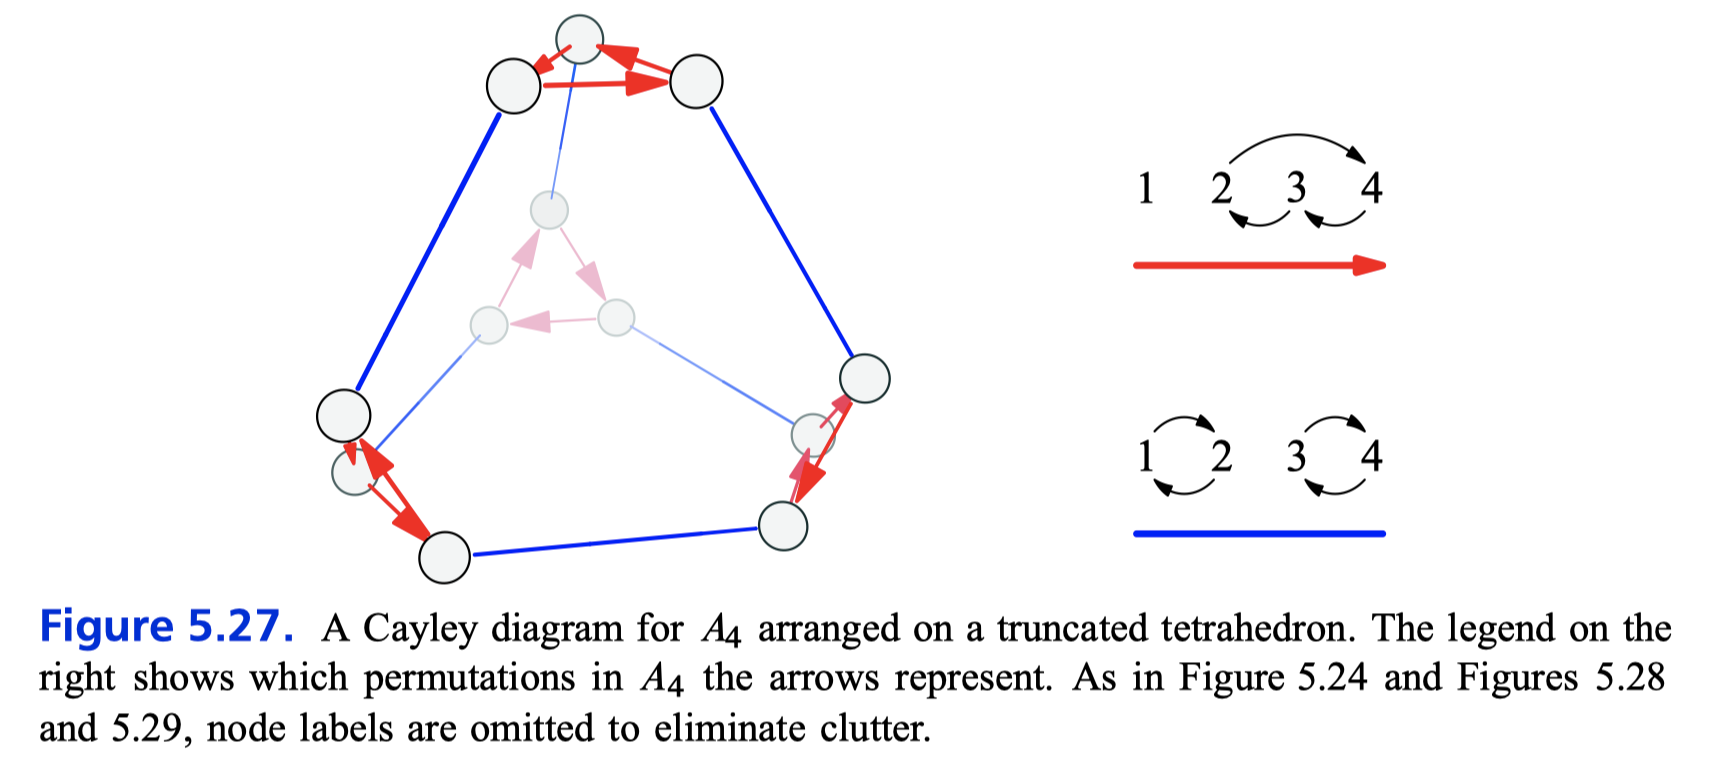
\includegraphics[width=1\textwidth]{fig/Group/Cayley-A4.png}
\end{figure}
(对比$A_4$和$S_4$的区别)

\begin{framed}
%\verb|\documentstyle[ifthen,12pt,titlepage]{article}|
\small{
通过对元素进行置换(permutation),可以很容易构成群;对$n$个元素进行全排列,构成对称群$S_n$;取其中一半的元素,构成$A_n$。
}
\end{framed}

\subsection{常见群的特点总结}
\begin{mdframed}[
linecolor=black!40,outerlinewidth=1pt,roundcorner=.5em,innertopmargin=1ex,innerbottommargin=.5\baselineskip,innerrightmargin=1em,innerleftmargin=1em,backgroundcolor=gray!5,
%backgroundcolor=blue!10,%userdefinedwidth=1\textwidth,%shadow=true,%shadowsize=6,%shadowcolor=black!20,%frametitle={The \textit{two-step} model of XMCD:},%frametitlebackgroundcolor=cyan!40,%frametitlerulewidth=10pt
]
\begin{enumerate}
\setlength{\itemsep}{0pt}
\setlength{\parsep}{0pt}
\setlength{\parskip}{0pt}
    \item \textbf{反演群$V_n$}:包含$n$个元素;
    \item \textbf{循环群$C_n$}:描述物体的旋转对称性,包含$n$个元素;也可以理解为对元素进行模加运算;
    \item \textbf{二面体群$D_n$}:二面体群不止描述旋转对称性,还描述了左右对称性(bilateral symmetry),包含$2n$个元素;
    \item \textbf{阿贝尔群(Abelian Group)}:满足结合律的群;所有的循环群都是阿贝尔群;阿贝尔群的乘法表是关于对角线对称的;
    \item \textbf{对称群$S_n$}:全体元素的全排列得到的群,包含$n!$个元素;
    \item \textbf{交错群$A_n$}:取$S_n$中一半元素构成的群,包含$n!/2$个元素;交错群$A_n$是对称群$S_n$的子群;交错群$A_n$是阿贝尔群,当且仅当$n \le 3$;
\end{enumerate}
\end{mdframed}

\subsection{置换(permutation)与群的关系}
对元素进行置换(permutation)运算,可以构成任意群;

以$S_3$为例,也可以理解为它是对元素进行了置换,如下图:
\begin{figure}[H]
    \centering
    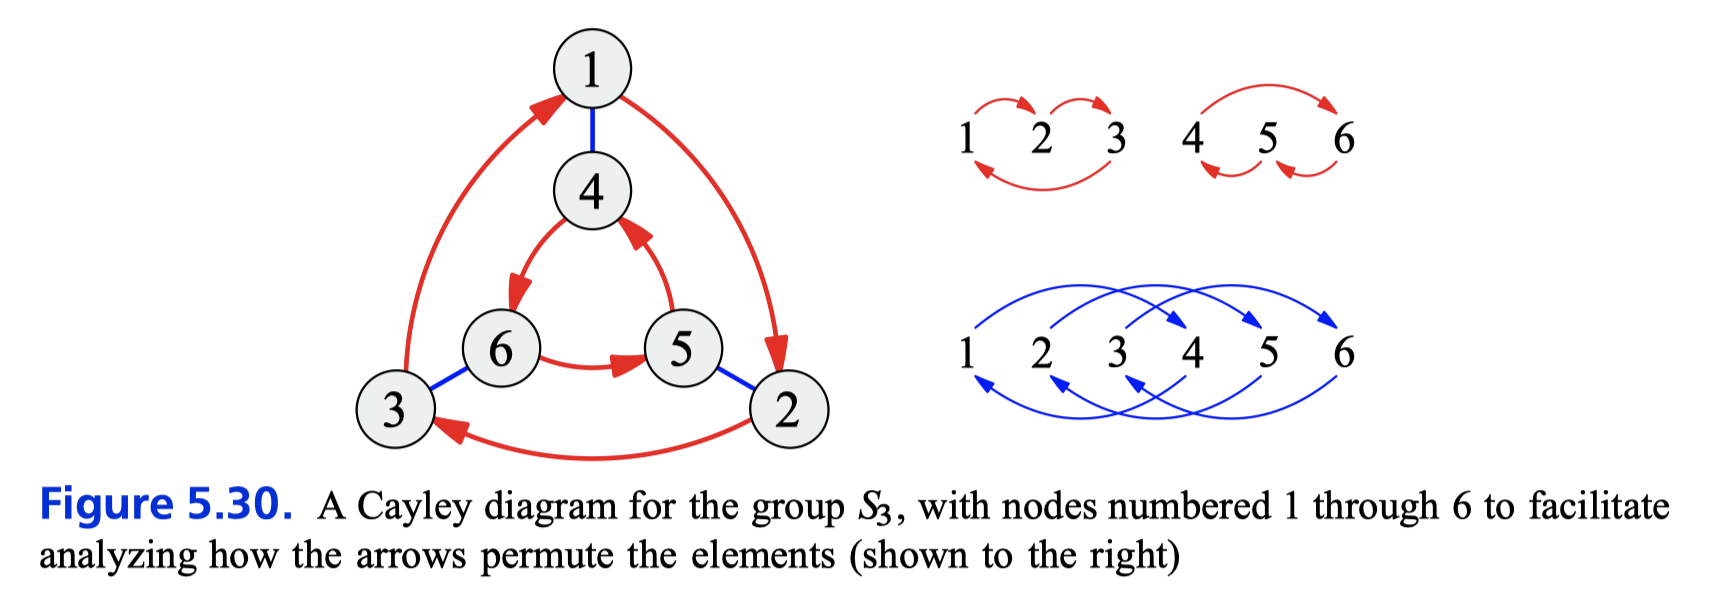
\includegraphics[width=1\textwidth]{fig/Group/Cayley-Permutation-S3.png}
\end{figure}

从反演群$V_4$的乘法表也可以看出它和元素置换的关系,如下图:
\begin{figure}[H]
    \centering
    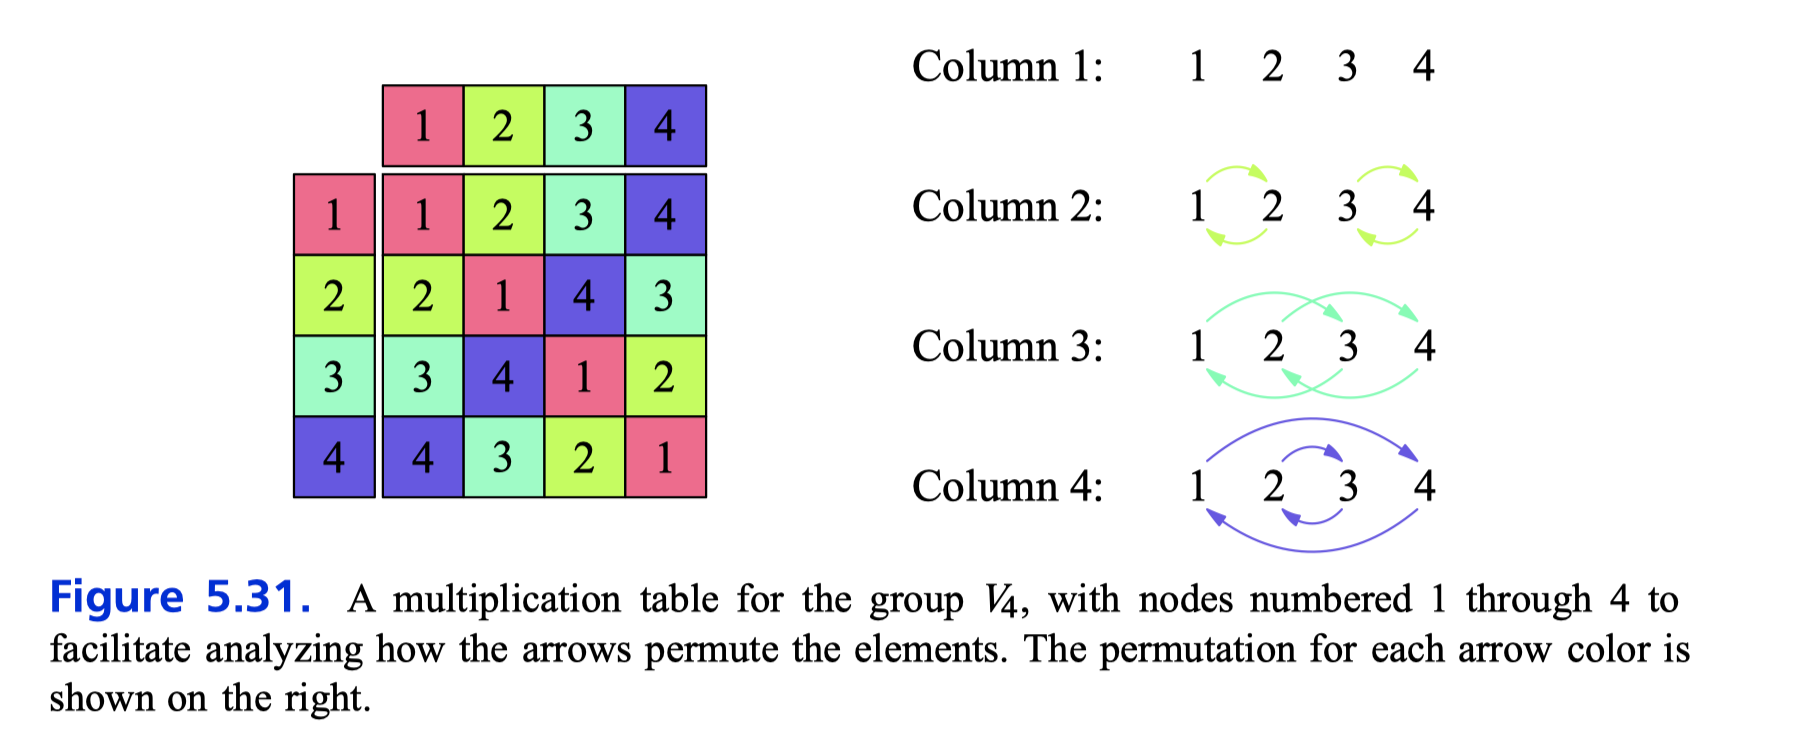
\includegraphics[width=1\textwidth]{fig/Group/Multiplication-Permutation-V4.png}
\end{figure}

\subsection{Cayley 定理(Cayley Theorem)}
每个群都与一类置换集合是同构的(Every group is isomorphic to a collection of permutations)。

\section{群的结构}
\subsection{循环群和群的生成元(generator)}
\begin{mdframed}[
linecolor=black!40,outerlinewidth=1pt,roundcorner=.5em,innertopmargin=1ex,innerbottommargin=.5\baselineskip,innerrightmargin=1em,innerleftmargin=1em,backgroundcolor=gray!5,
%backgroundcolor=blue!10,%userdefinedwidth=1\textwidth,%shadow=true,%shadowsize=6,%shadowcolor=black!20,%frametitle={The \textit{two-step} model of XMCD:},%frametitlebackgroundcolor=cyan!40,%frametitlerulewidth=10pt
]
循环群的定义:对于$n$阶群$G$,如果存在$a \in G$,使得$G = \{a^0, a, a^2, \cdots, a^{n-1}\}$,则称$G$为由$a$生成的(有限)循环群,记作$G = \langle a \rangle$,$a$是$G$的一个生成元{\cite{From_Linear_Equation_To_Galois_Theory}}。
\end{mdframed}
根据\cite{Visual_Group_Theory},生成元不只针对循环群,例如,可以说$V_4$的生成元是$\langle R, B \rangle$;$C_6 = \{0, 1, 2, 3, 4, 5\}$可以由如下生成元生成;$\langle 1 \rangle, \langle 5 \rangle, \langle 2, 3 \rangle$
\begin{figure}[H]
    \centering
    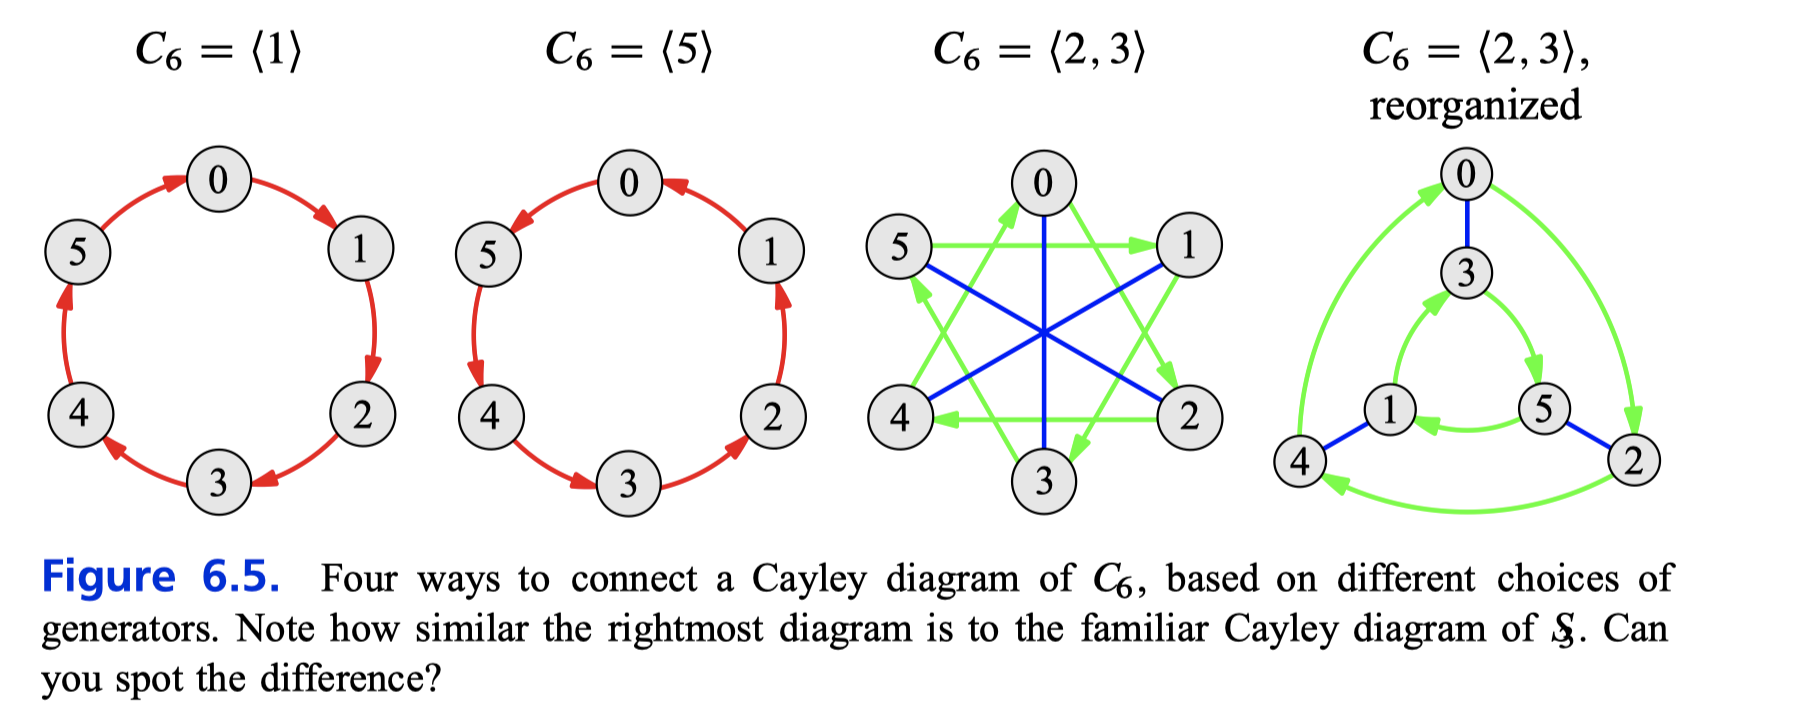
\includegraphics[width=1\textwidth]{fig/Group/Cayley-C6-Generators.png}
\end{figure}


\subsection{子群(Subgroup)}
\begin{mdframed}[
linecolor=black!40,outerlinewidth=1pt,roundcorner=.5em,innertopmargin=1ex,innerbottommargin=.5\baselineskip,innerrightmargin=1em,innerleftmargin=1em,backgroundcolor=gray!5,
%backgroundcolor=blue!10,%userdefinedwidth=1\textwidth,%shadow=true,%shadowsize=6,%shadowcolor=black!20,%frametitle={The \textit{two-step} model of XMCD:},%frametitlebackgroundcolor=cyan!40,%frametitlerulewidth=10pt
]
子群在不同资料中的定义:

如果一个群完全包含在另一个群中,称被包含的群为其子群;如果$H$是$G$的子群,记作:$H < G${\cite{Visual_Group_Theory}}

群$G$的非空子集合$H$称为$G$的一个子群,记作$H \unlhd G$,或$G \unrhd H$(原书符号无法打出,类似这样),如果在$G$所定义的乘法运算下,$H$本身构成构成一个群。{\cite{From_Linear_Equation_To_Galois_Theory}}
\end{mdframed}

子群的Cayley图如下:
\begin{figure}[H]
    \centering
    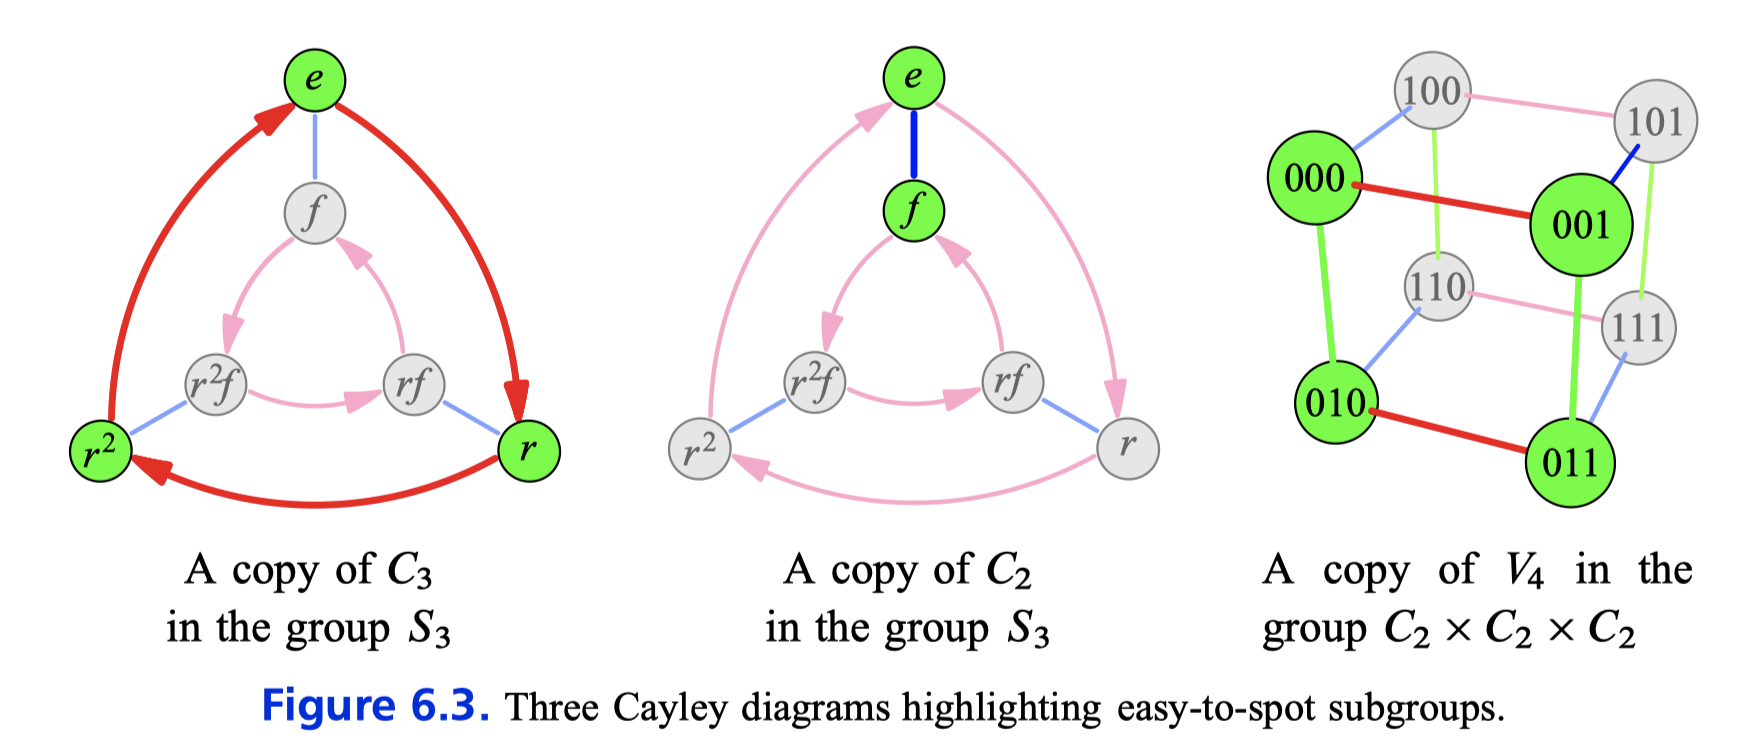
\includegraphics[width=.8\textwidth]{fig/Group/Cayley-Subgroup.png}
\end{figure}

显然,$\{e\}$和$G$本身都是$G$的子群,它们是$G$的\textbf{平凡子群}。$G$的其它子群则是$G$的\textbf{真子群}。

\begin{mdframed}[
linecolor=black!40,outerlinewidth=1pt,roundcorner=.5em,innertopmargin=1ex,innerbottommargin=.5\baselineskip,innerrightmargin=1em,innerleftmargin=1em,backgroundcolor=gray!5,
%backgroundcolor=blue!10,%userdefinedwidth=1\textwidth,%shadow=true,%shadowsize=6,%shadowcolor=black!20,%frametitle={The \textit{two-step} model of XMCD:},%frametitlebackgroundcolor=cyan!40,%frametitlerulewidth=10pt
]
\textbf{
子群的判断定理:设 $H \subseteq G$,$H$是$G$的子群的充要条件是对任意$a, b \in H$,有$ab^{-1} \in H$
}
\end{mdframed}

\begin{framed}
%\verb|\documentstyle[ifthen,12pt,titlepage]{article}|
\small{
理解:$H$若想成为$G$的子群,需要满足的条件,是对于任意$a,b \in H$,有$ab^{-1} \in H$,即$a$“乘法运算”$b$的逆得到的元,仍然在$H$中。
}
\end{framed}

\subsection{陪集(Coset)}
用 $G$的真子群$H$来给出$G$的一个\textbf{分类}。由$H \subset G$,可知存在$a_2 \in G - H$($G$和$H$的差集),于是构造:
$$
a_2H = \{a_2h | h \in H\}
$$

容易证明,$H \cap a_2H = \varnothing$。如果存在$a_3 \in G$,且$a_3 \notin H\cup a_2H$,则同样再构造$a_3H$,也有$a_3H \cap (H \cup a_2H) = \varnothing$。类似地,可得到$a_4H, a_5H, \cdots$,于是当群$G$是有限群时,就有:
$$
G = H \cup a_2H \cup a_3H \cup \cdots a_lH
$$

我们把$G$的具有$aH$形式的子集,称为$G$的关于子群$H$的由元素$a$给出的\textbf{左陪集}。令$a_1 = e$,由$H = eH = a_1H$可知,$H$也是$G$的一个左陪集。于是上式$G = H \cup a_2H \cup a_3H \cup \cdots a_lH$称为$G$的一个\textbf{左陪集分解}。

陪集可以看做是子群的拷贝(copy),如下图所示:
\begin{figure}[H]
    \centering
    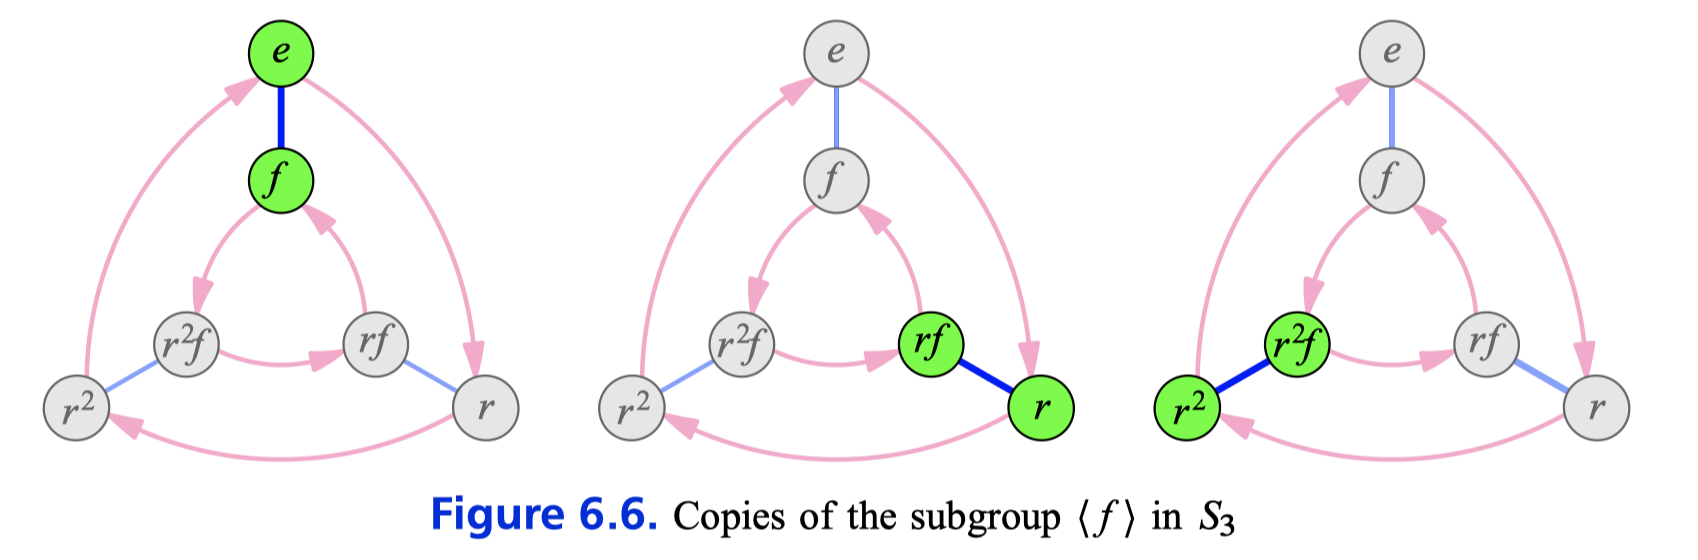
\includegraphics[width=1\textwidth]{fig/Group/Cayley-Copy-Of-Subgroup.png}
\end{figure}
左边的图是子群$\langle f \rangle = \{e, f\}$,中间和右边的集合 $\{r, rf\}, \{r^2, r^2f\}$不是群(因为它们不包含单位元),但是结构和$\langle f \rangle$相同,叫做陪集。

\begin{framed}
%\verb|\documentstyle[ifthen,12pt,titlepage]{article}|
每个子群都有陪集,所有的陪集覆盖了Cayley图的每一个元素(Every subgroup has cosets, and they cover every node of the group's Cayley diagram )
\end{framed}

\subsubsection{基于Cayley图理解左右陪集}
根据陪集的定义,有:
$$
r \langle f \rangle = r \{ e, f \} = \{ r \cdot e, r \cdot f\} = \{r, rf\}
$$
$$
\langle f \rangle r = \{ e, f \} r = \{ e \cdot r, f \cdot r\} = \{r, r^2f\}
$$

\textbf{从Cayley图上来看,左陪集$r \langle f \rangle $可以看成从节点$r$出发,进行$f$运算得到的集合;右陪集$\langle f \rangle r$可以看成从子集$\langle f \rangle $出发,对其中的每个元素进行$r$运算得到的集合}。
\begin{figure}[H]
    \centering
    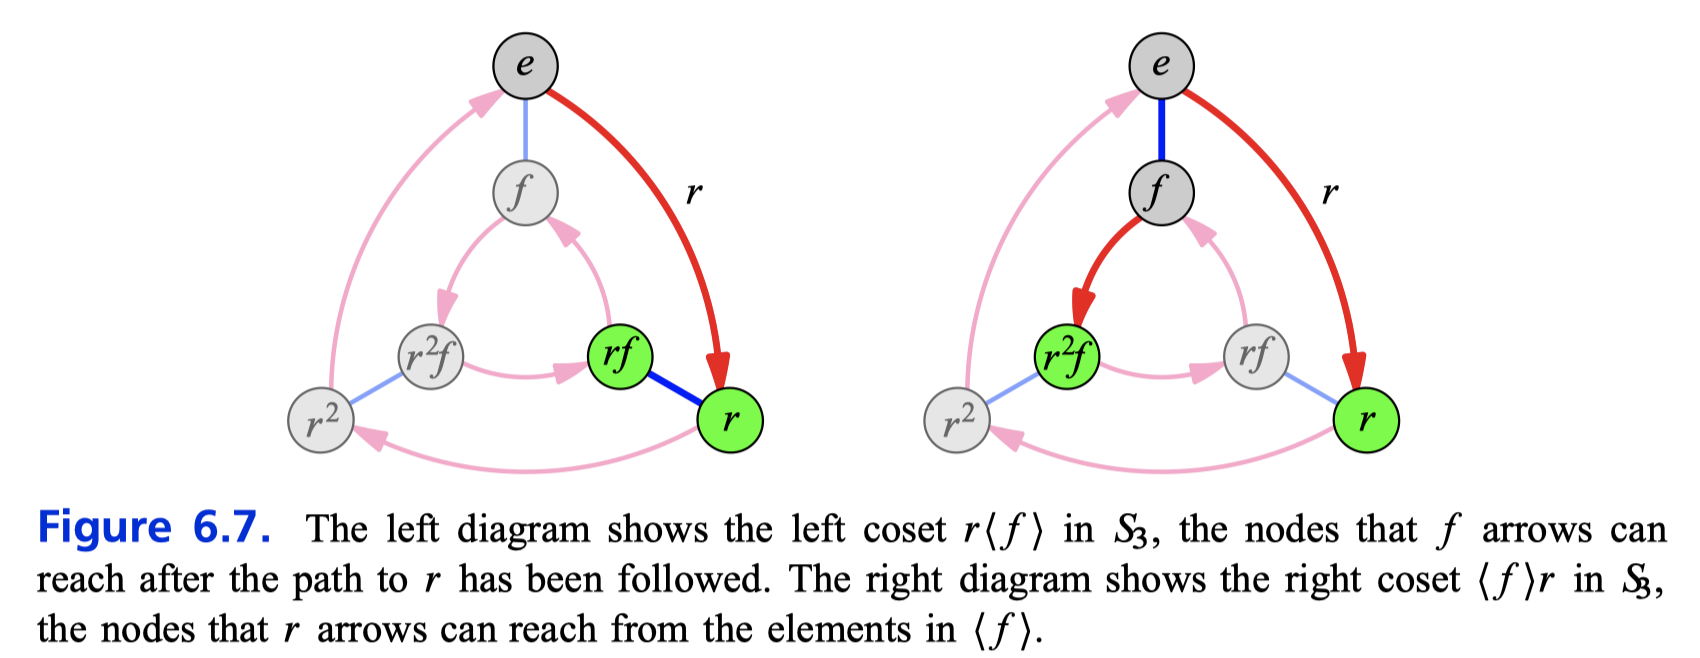
\includegraphics[width=1\textwidth]{fig/Group/Cayley-Left-Right-Cosets.png}
\end{figure}
\begin{figure}[H]
    \centering
    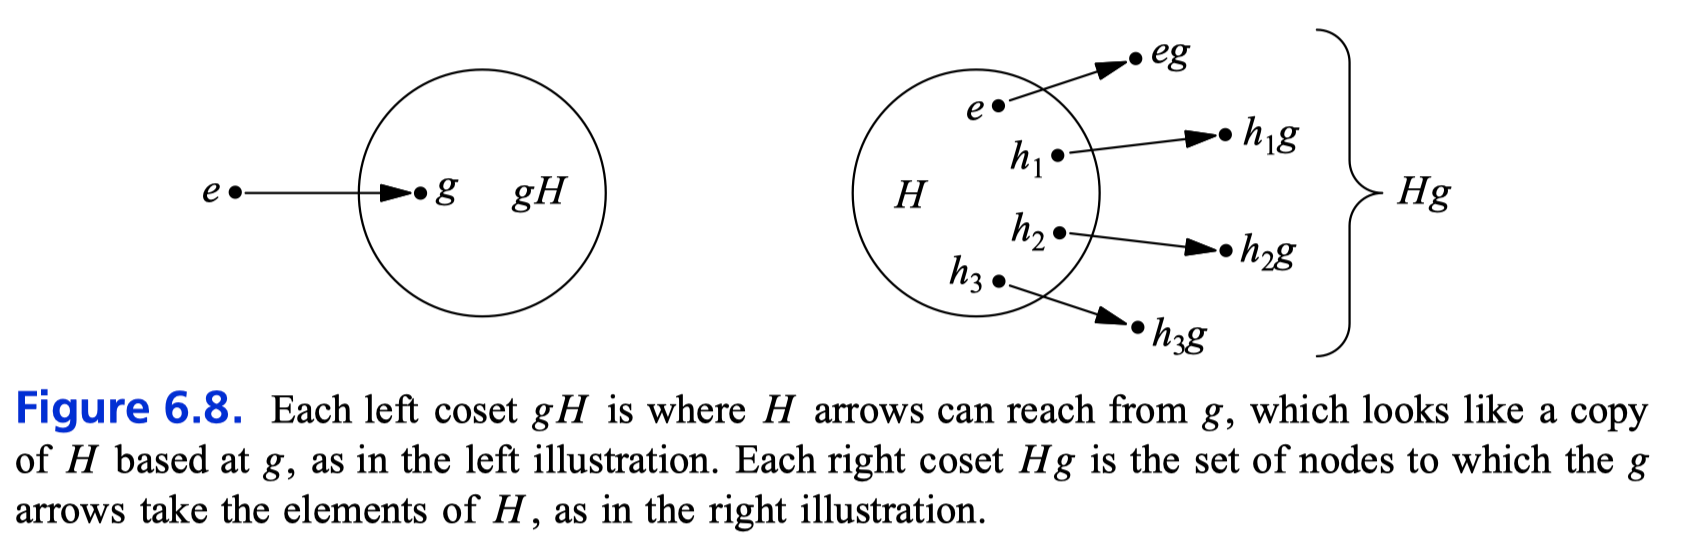
\includegraphics[width=1\textwidth]{fig/Group/Compare-Left-Right-Cosets.png}
\end{figure}

\subsection{拉格朗日定理(Lagrange's Theorem)}
如果$H$是$G$的子群,那么$G$的每个元素都属于并且只属于$H$的一个陪集。

\begin{mdframed}[
linecolor=black!40,outerlinewidth=1pt,roundcorner=.5em,innertopmargin=1ex,innerbottommargin=.5\baselineskip,innerrightmargin=1em,innerleftmargin=1em,backgroundcolor=gray!5,
%backgroundcolor=blue!10,%userdefinedwidth=1\textwidth,%shadow=true,%shadowsize=6,%shadowcolor=black!20,%frametitle={The \textit{two-step} model of XMCD:},%frametitlebackgroundcolor=cyan!40,%frametitlerulewidth=10pt
]
\textbf{
拉格朗日定理(Lagrange's Theorem):如果$H < G$($H$是$G$的子集),则$H$的阶(order)$|H|$能被$|G|$整除。
}
\end{mdframed}

所以,群可以看成是由其子群和对应的陪集组合而成;如下图:
\begin{figure}[H]
    \centering
    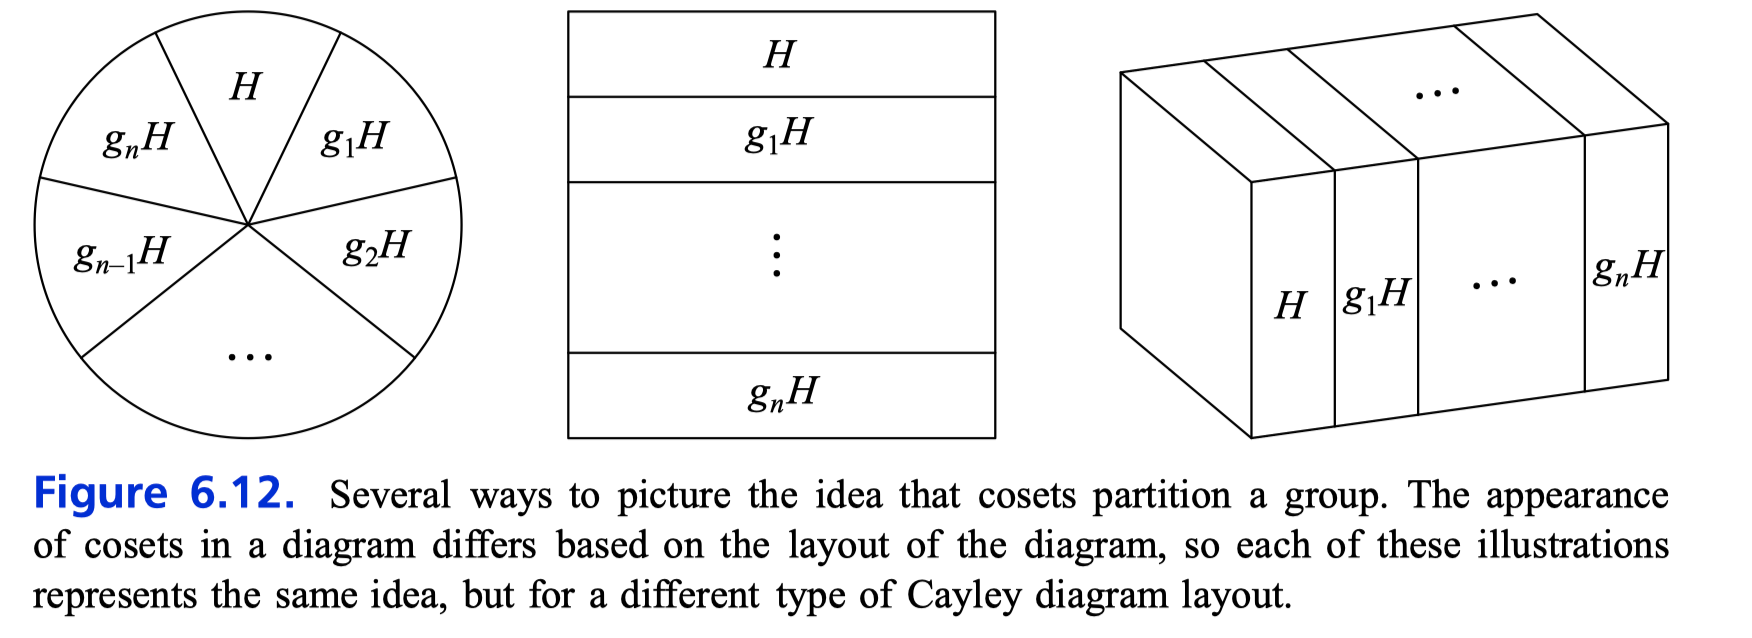
\includegraphics[width=1\textwidth]{fig/Group/Group-Decomposition.png}
\end{figure}


\subsection{正规子群}
\begin{mdframed}[
linecolor=black!40,outerlinewidth=1pt,roundcorner=.5em,innertopmargin=1ex,innerbottommargin=.5\baselineskip,innerrightmargin=1em,innerleftmargin=1em,backgroundcolor=gray!5,
%backgroundcolor=blue!10,%userdefinedwidth=1\textwidth,%shadow=true,%shadowsize=6,%shadowcolor=black!20,%frametitle={The \textit{two-step} model of XMCD:},%frametitlebackgroundcolor=cyan!40,%frametitlerulewidth=10pt
]
\textbf{
正规子群的定义:如果$G$的子群$H$,对任意$a \in G$,满足$aH = Ha$,即此时不必区分左右陪集,则称$H$为$G$的一个正规子群,记作 $G \rhd H$或$H \lhd G$。
}
\end{mdframed}

\subsection{单群}

\section{群上的运算}
\subsection{直积(direct product)}
\begin{mdframed}[
linecolor=black!40,outerlinewidth=1pt,roundcorner=.5em,innertopmargin=1ex,innerbottommargin=.5\baselineskip,innerrightmargin=1em,innerleftmargin=1em,backgroundcolor=gray!5,
%backgroundcolor=blue!10,%userdefinedwidth=1\textwidth,%shadow=true,%shadowsize=6,%shadowcolor=black!20,%frametitle={The \textit{two-step} model of XMCD:},%frametitlebackgroundcolor=cyan!40,%frametitlerulewidth=10pt
]
基于Cayley图,构造两个群$A,B$直积$A\times B$的直观方法:
\begin{enumerate}
\setlength{\itemsep}{0pt}
\setlength{\parsep}{0pt}
\setlength{\parskip}{0pt}
	\item 对$A$的每个节点“充气(inflate)”,在其中拷贝入$B$的Cayley图
	\item 删除“充气”后的$A$节点,用原来$A$节点的对应关系,连接上新拷贝的$B$的对应节点
\end{enumerate}

Technique for constructing direct product using Cayley diagram. To create a Cayley diagram for $A \times B$ from Cayley diagram of A and B, proceed as follows.
\begin{enumerate}
\setlength{\itemsep}{0pt}
\setlength{\parsep}{0pt}
\setlength{\parskip}{0pt}
	\item Begin with the Cayley diagram for A.
	\item Inflate each node in the Cayley diagram of A and place in it a copy of the Cayley diagram for B.
	\item Remove the (inflated) nodes of A while using the arrows of A to connect corresponding nodes from each copy of B. That is, remove the A diagram but treat its arrows as a blueprint for how to connect corresponding nodes in the copies of B.
\end{enumerate}
\end{mdframed}

直接上图:
\begin{figure}[H]
    \centering
    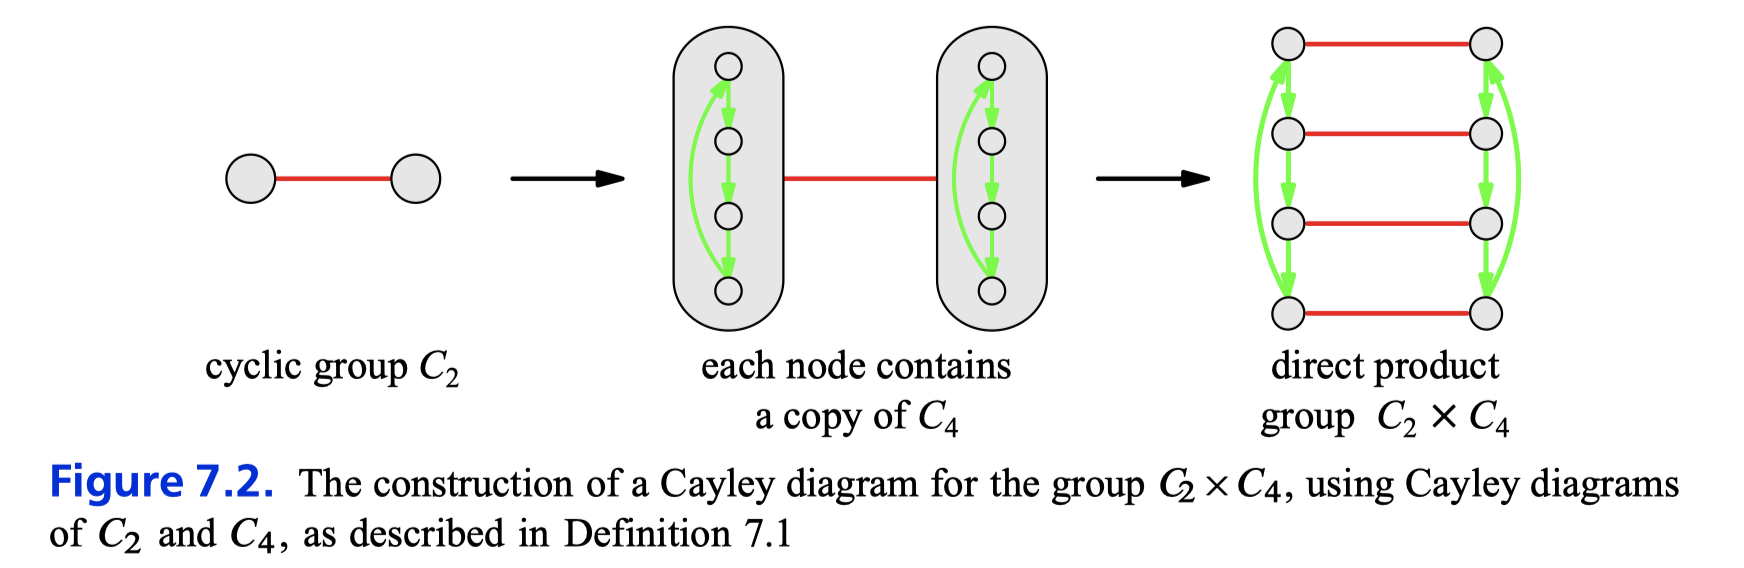
\includegraphics[width=1\textwidth]{fig/Group/Cayley-C2-times-C4.png}
\end{figure}
\begin{figure}[H]
    \centering
    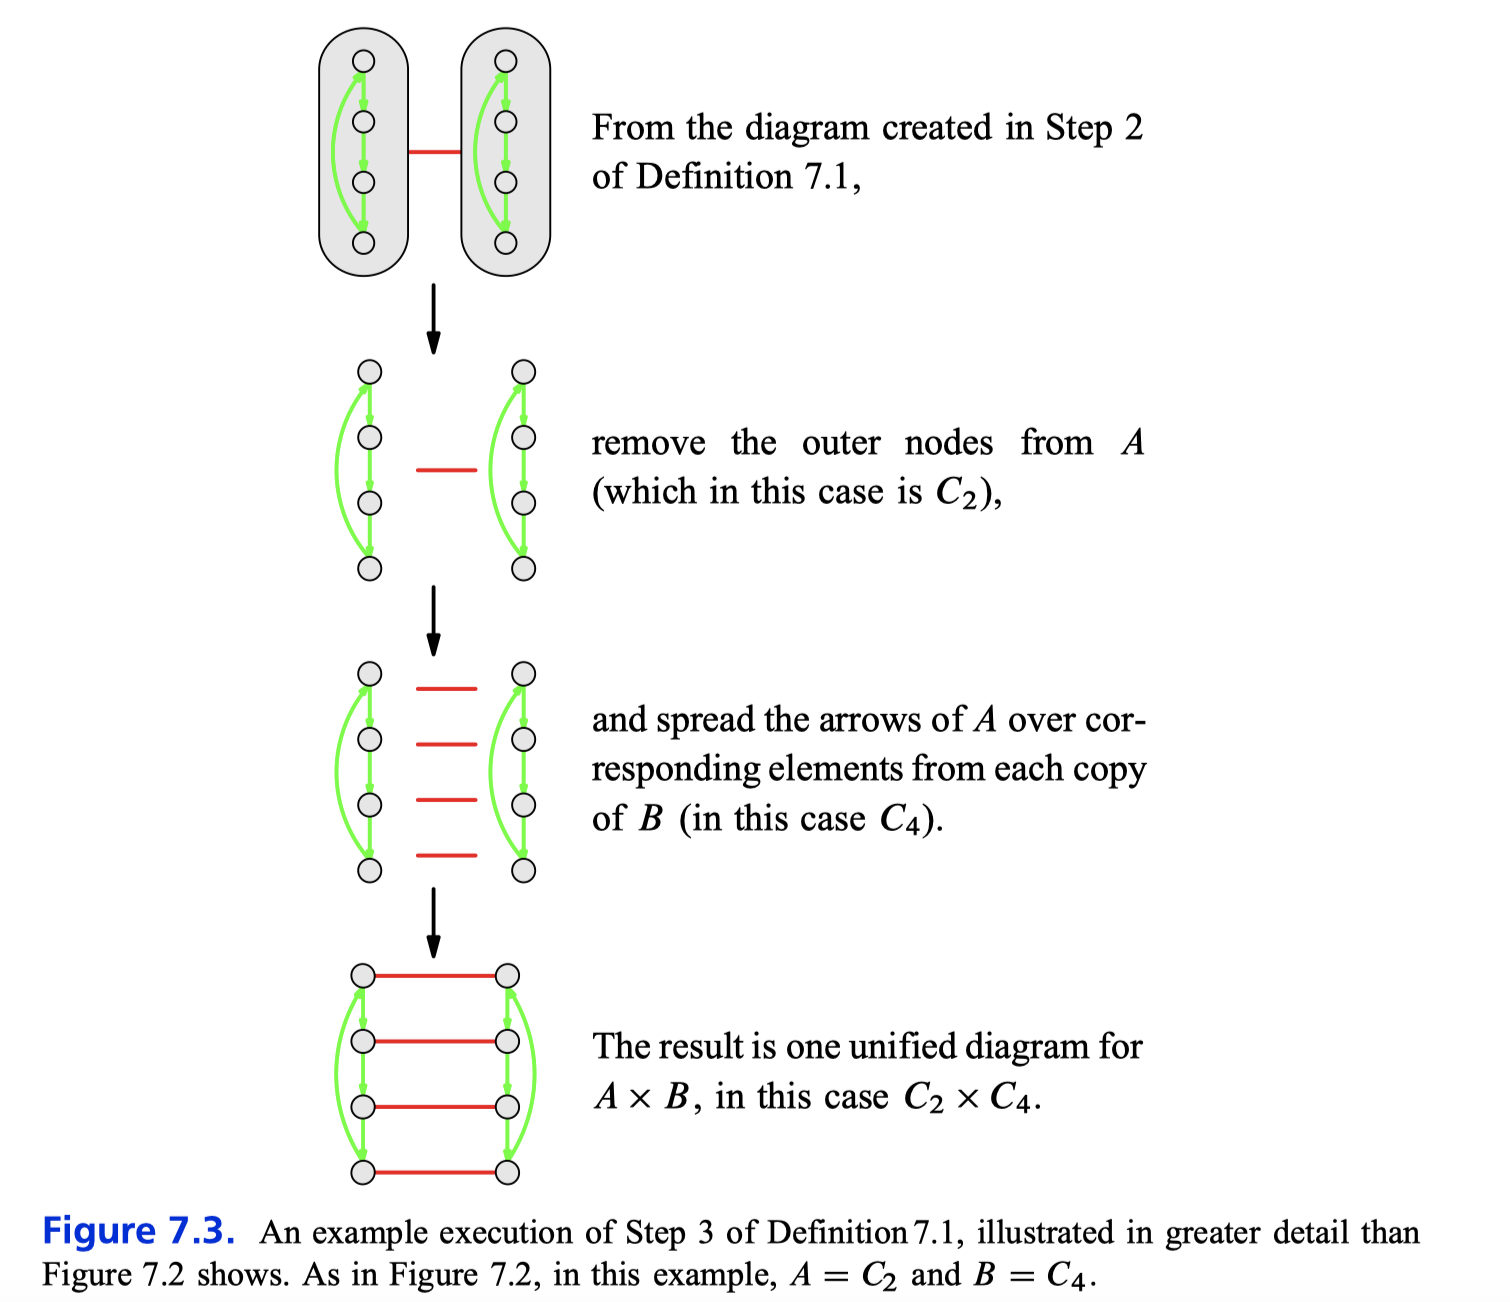
\includegraphics[width=1\textwidth]{fig/Group/Cayley-C2-times-C4-detailed.png}
\end{figure}
\begin{figure}[H]
    \centering
    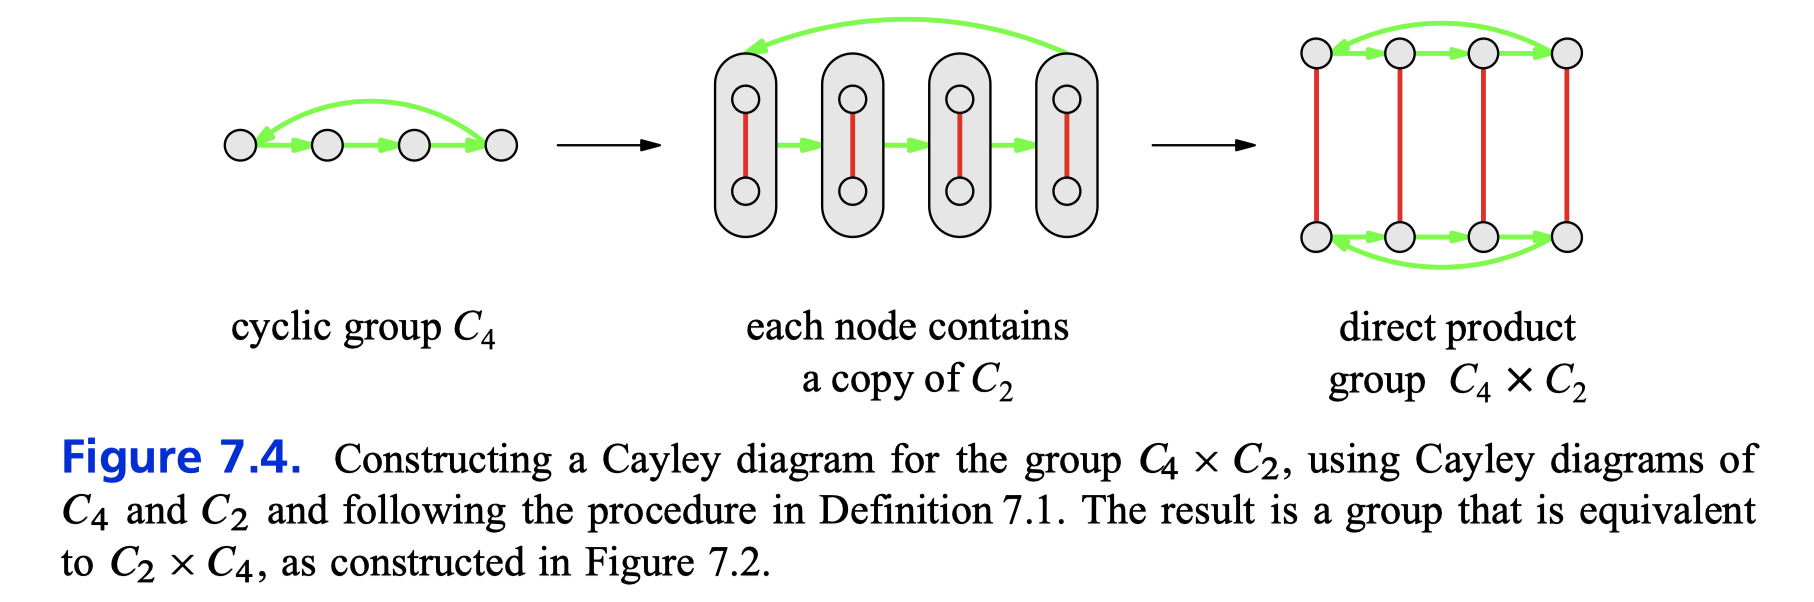
\includegraphics[width=1\textwidth]{fig/Group/Cayley-C4-times-C2.png}
\end{figure}
\begin{figure}[H]
    \centering
    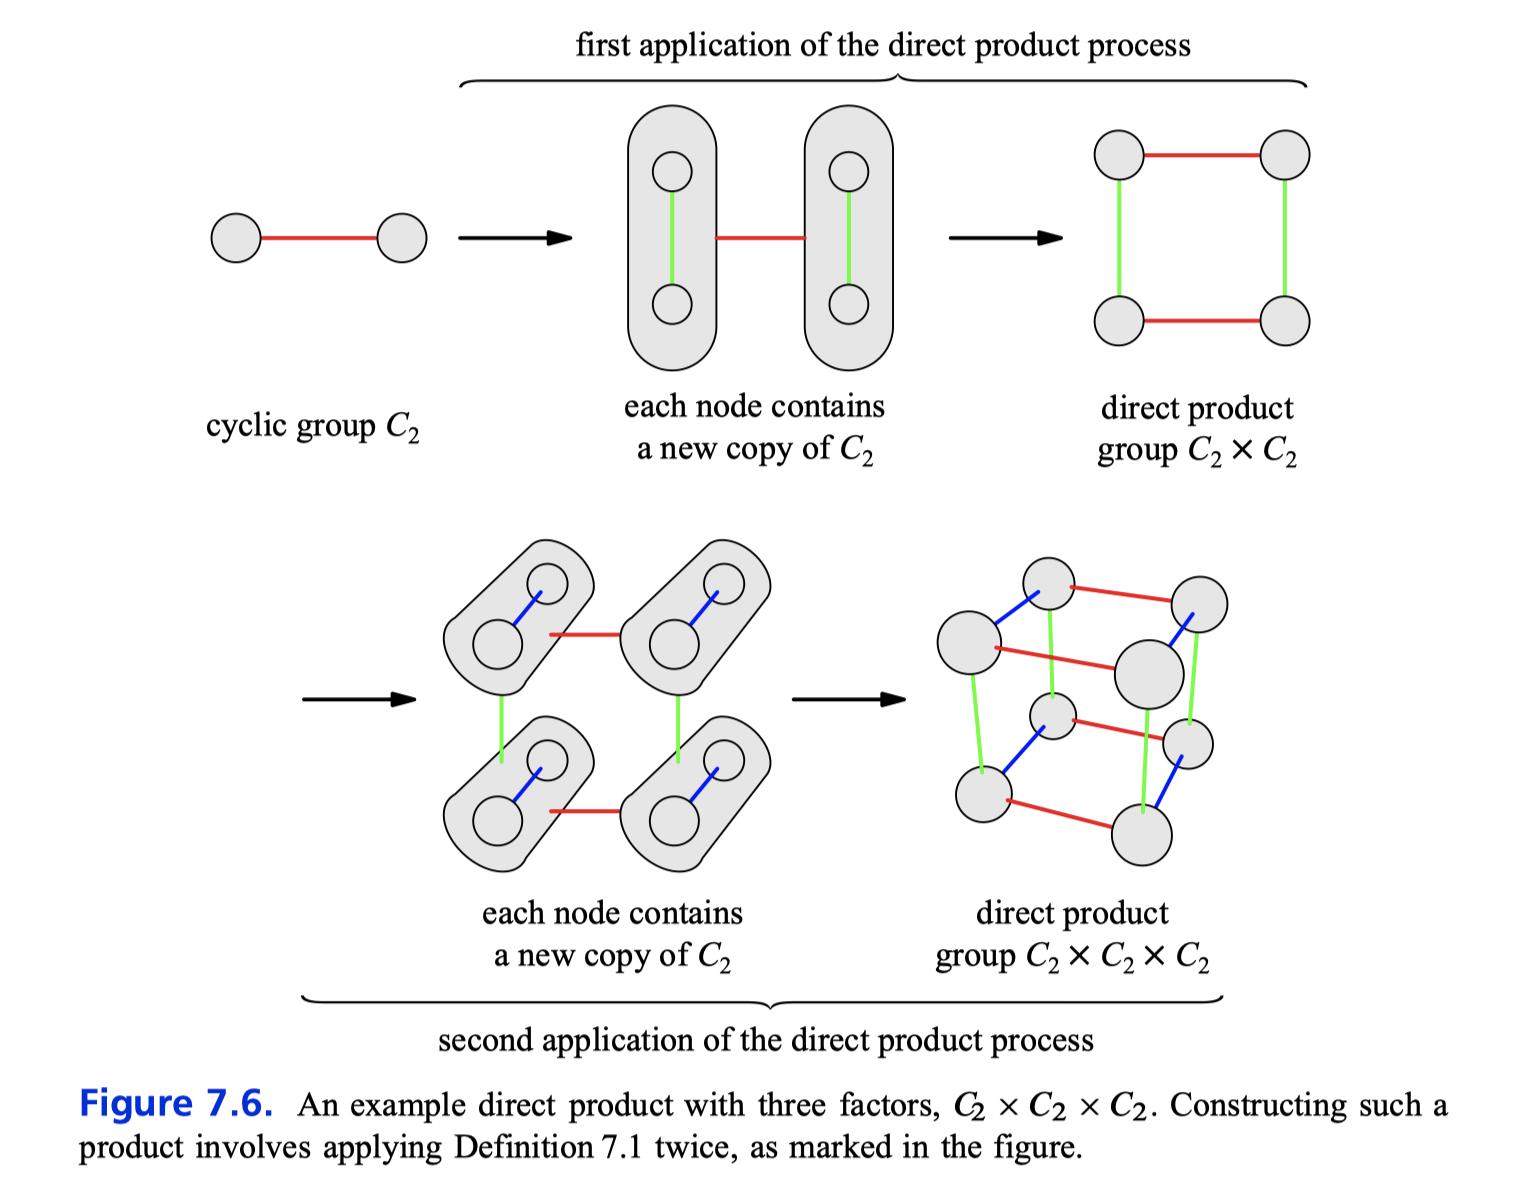
\includegraphics[width=1\textwidth]{fig/Group/Cayley-C2-times-C2-times-C2.png}
\end{figure}
\begin{figure}[H]
    \centering
    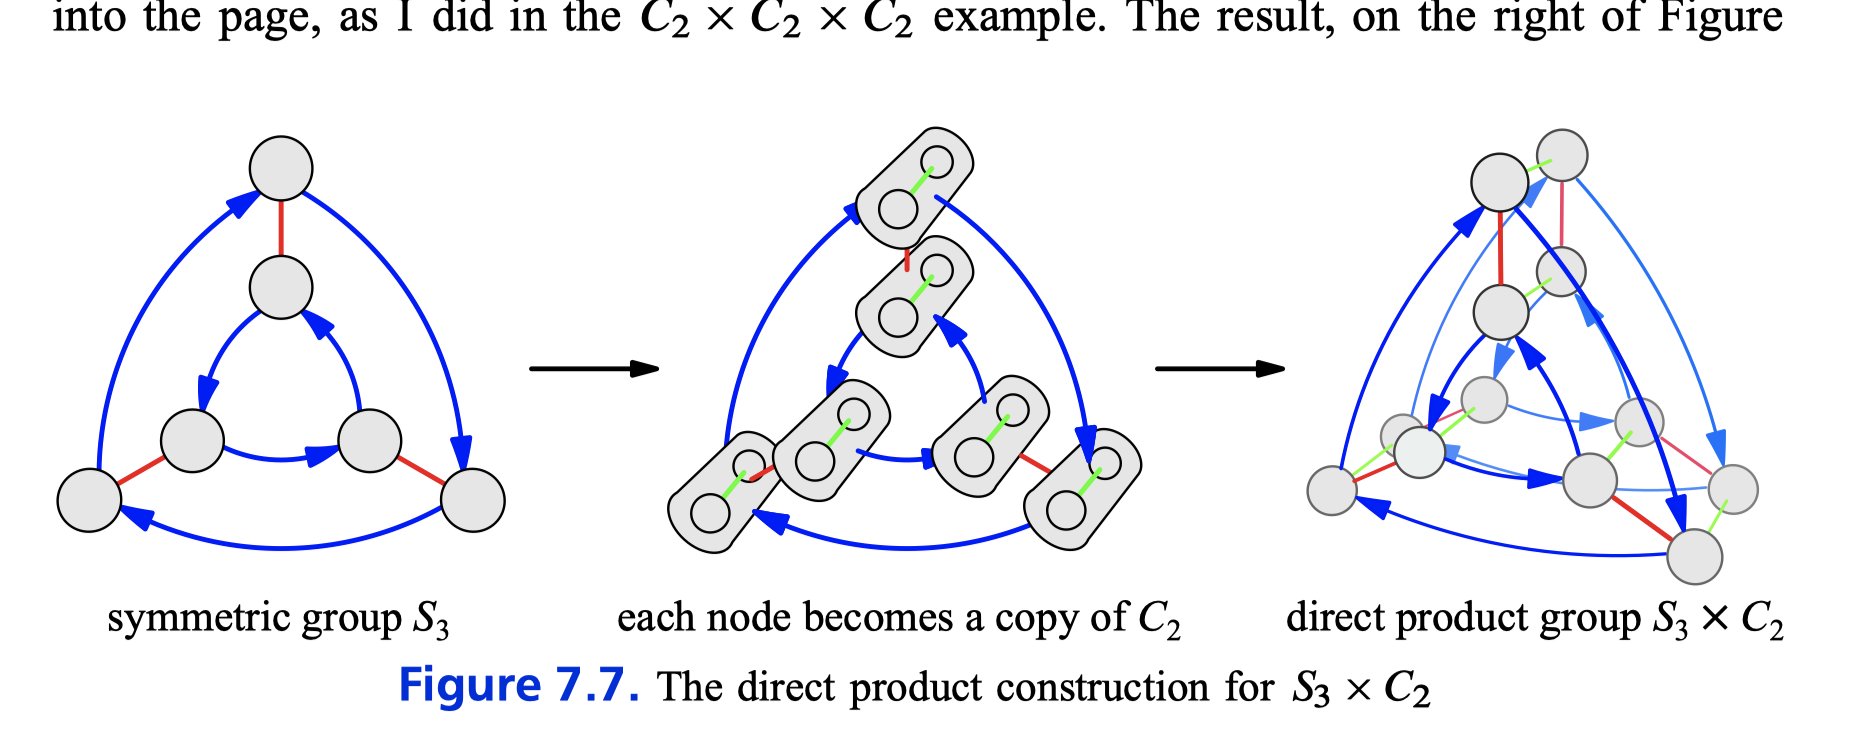
\includegraphics[width=1\textwidth]{fig/Group/Cayley-S3-times-C2.png}
\end{figure}

做直积后,节点的命名方式:
\begin{figure}[H]
    \centering
    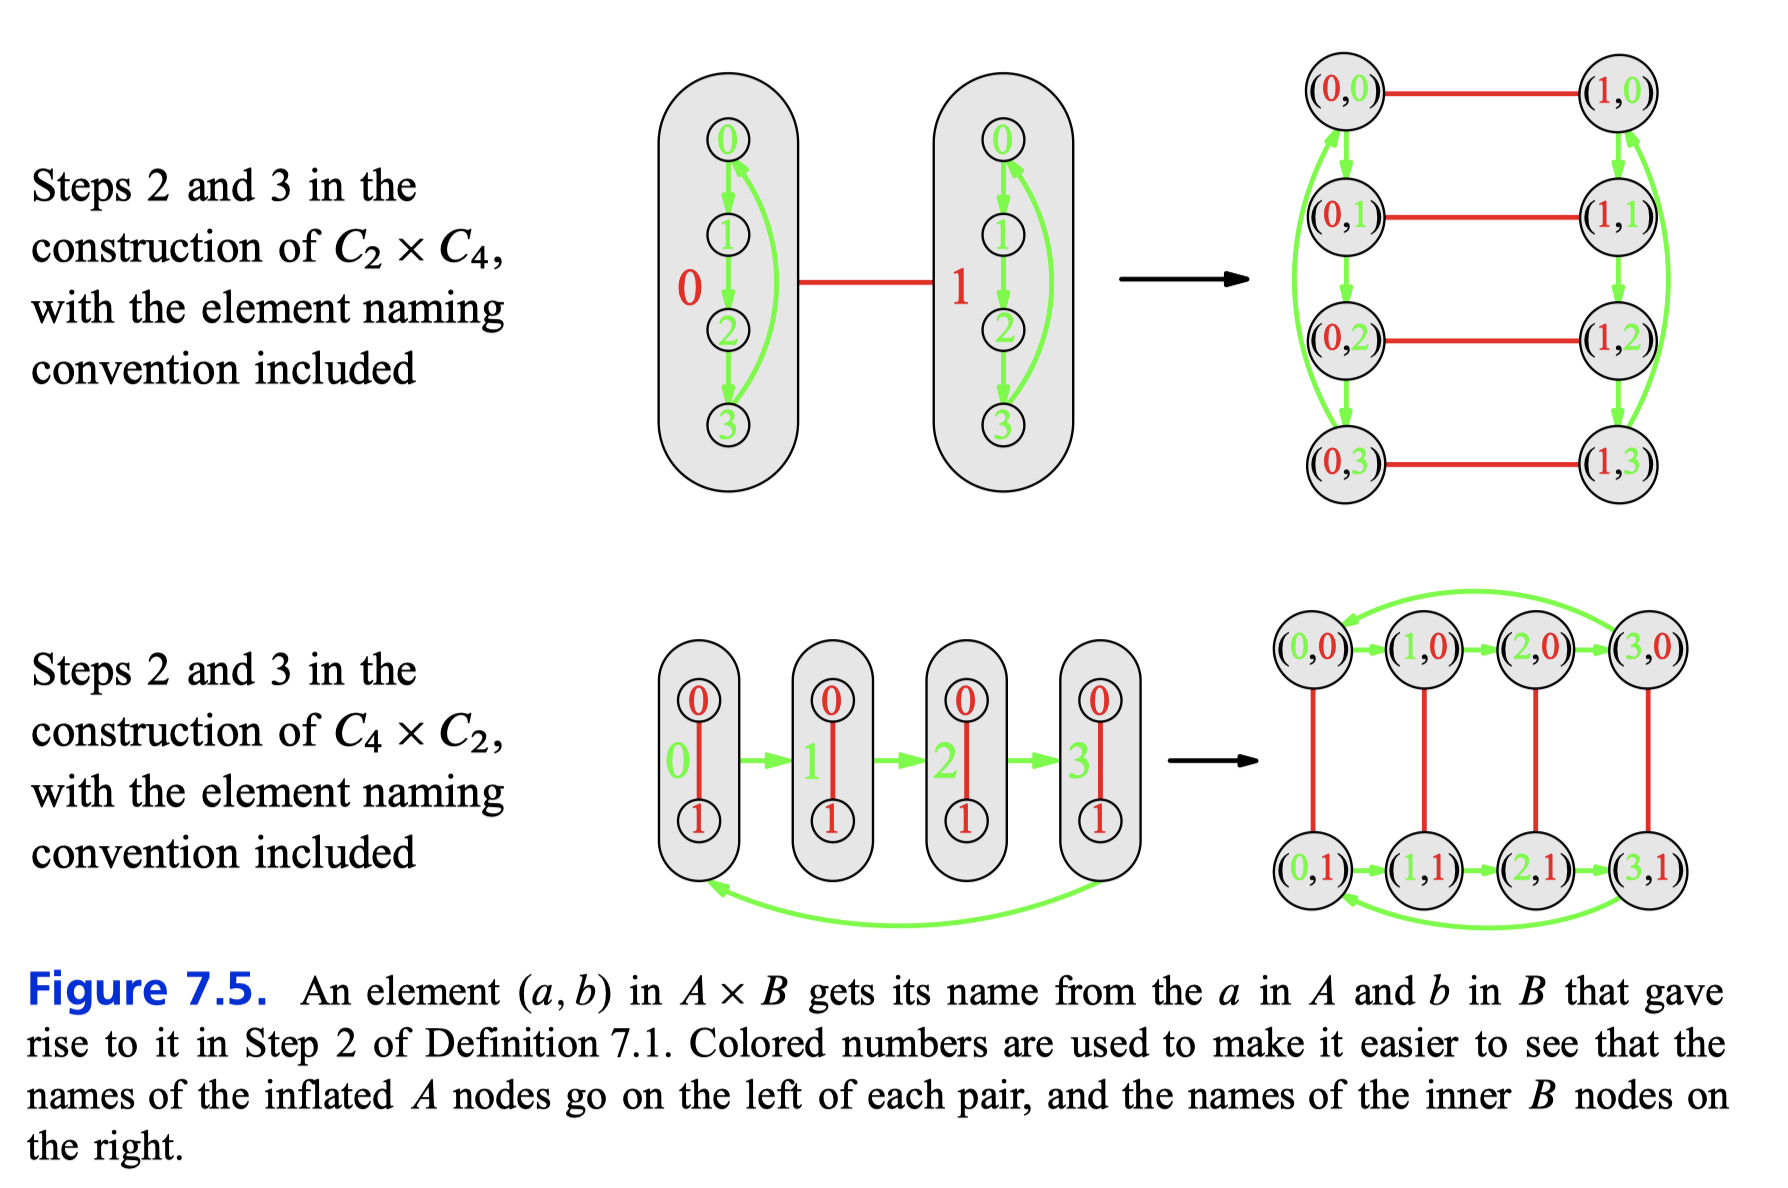
\includegraphics[width=1\textwidth]{fig/Group/Cayley-Direct-Product-Naming.png}
\end{figure}

\begin{mdframed}[
linecolor=black!40,outerlinewidth=1pt,roundcorner=.5em,innertopmargin=1ex,innerbottommargin=.5\baselineskip,innerrightmargin=1em,innerleftmargin=1em,backgroundcolor=gray!5,
%backgroundcolor=blue!10,%userdefinedwidth=1\textwidth,%shadow=true,%shadowsize=6,%shadowcolor=black!20,%frametitle={The \textit{two-step} model of XMCD:},%frametitlebackgroundcolor=cyan!40,%frametitlerulewidth=10pt
]
\textbf{
对于任意群$A,B$,总有:$A \lhd A \times B$ 和 $B \lhd A \times B$,即$A$和$B$是$A \times B$的正规子群
}
\end{mdframed}

\begin{mdframed}[
linecolor=black!40,outerlinewidth=1pt,roundcorner=.5em,innertopmargin=1ex,innerbottommargin=.5\baselineskip,innerrightmargin=1em,innerleftmargin=1em,backgroundcolor=gray!5,
%backgroundcolor=blue!10,%userdefinedwidth=1\textwidth,%shadow=true,%shadowsize=6,%shadowcolor=black!20,%frametitle={The \textit{two-step} model of XMCD:},%frametitlebackgroundcolor=cyan!40,%frametitlerulewidth=10pt
]
基于乘法表构建直积的方式:
\begin{enumerate}
\setlength{\itemsep}{0pt}
\setlength{\parsep}{0pt}
\setlength{\parskip}{0pt}
	\item Begin with a multiplication table for $A$.
	\item Inflate each cell in the table to include a copy of the entire multiplication table for $B$. To avoid losing the information from the original table for $A$, retain its labels as well.
	\item Rename the elements in the table as pairs, using the $A$ elements on the left of each pair and the $B$ elements on the right.
\end{enumerate}
\end{mdframed}
\begin{figure}[H]
    \centering
    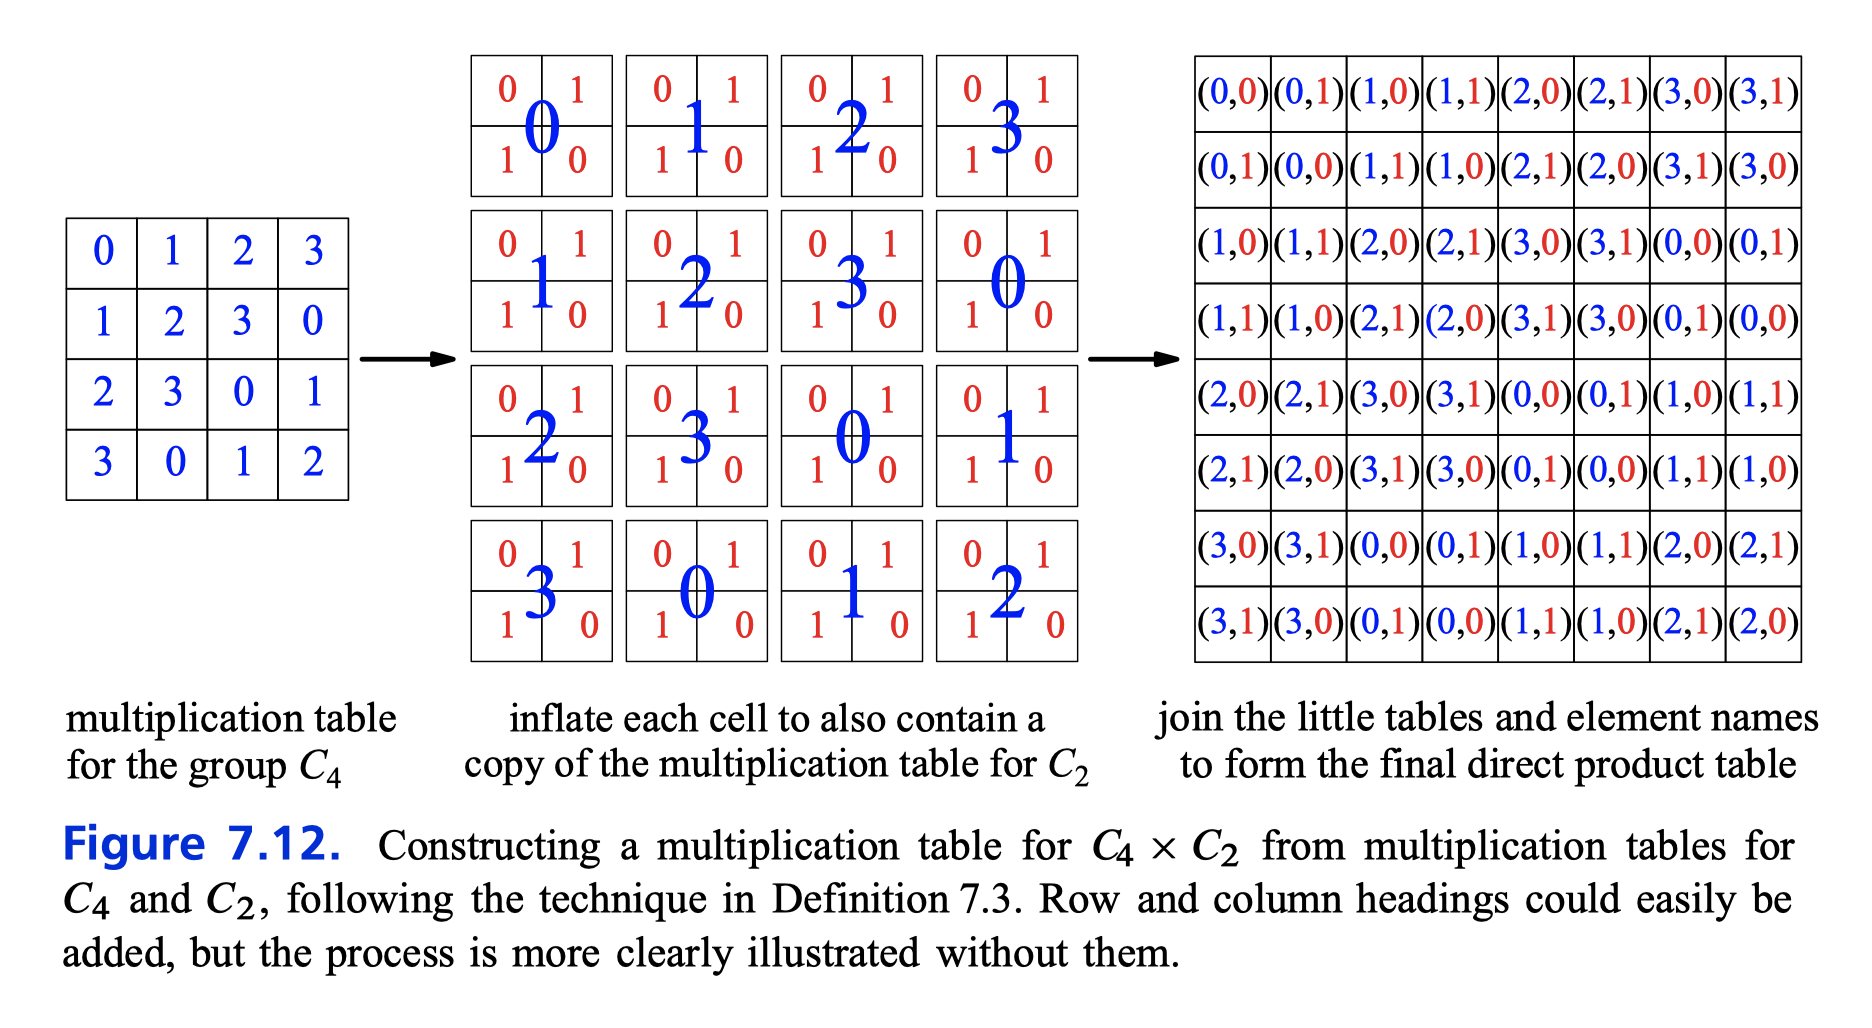
\includegraphics[width=1\textwidth]{fig/Group/MultiplicationTable-C4-times-C2.png}
\end{figure}

上图中,元素的具体计算过程举例:
$$
(2, 1) \cdot (3, 1)  = (2 + 3, 1 + 1) = (1, 0)
$$



\subsection{半直积(semidirect product)}
\subsection{商(quotient)}

homomorphism; isomorphism

\section{群的性质}

\subsection{阿贝尔群基础定理(Fundamental Theorem of Abelian Groups)}
第八章

\section{群相关概念的推演关系\cite{Introduction_Of_Algebra_Structure}}
\subsection{群}
代数结构(R, *),二元运算根据封闭性、单位元、逆元、结合律、交换律,可以归纳成不同的群。从最不严格到严格(依次添加限制条件),各种群的关系图如下:
\begin{figure}[H]
    \centering
    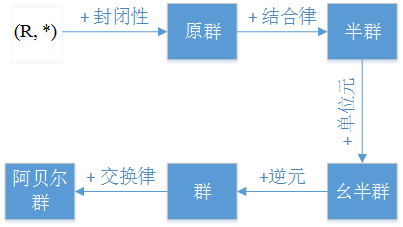
\includegraphics[width=0.5\textwidth]{fig/GroupLikeRelations.png}
\end{figure}

\subsubsection{原群(magma)}
原群(magma)是一种基本的代数结构,只要满足两元素作二元运算得到新元素仍属于该集合,即封闭性。

\subsubsection{半群(magma)}
半群(Semigroup),满足结合律(associative property)的代数结构。$V=<S,* >$,其中二元运算*是可结合的,即$(a*b)*c=a*(b*c)$,则称$V$是半群。

\subsubsection{幺半群(monoid)}
幺半群在半群的基础上,还需要满足有一个单位元。

\subsubsection{群(group)}
群(group)是两个元素作二元运算得到的一个新元素,需要满足群公理(group axioms),即:
\begin{itemize}
\setlength{\itemsep}{0pt}
\setlength{\parsep}{0pt}
\setlength{\parskip}{0pt}
\item 封闭性:$a ∗ b$仍然属于该集合
\item 结合律:$(a ∗ b) ∗ c = a ∗ (b ∗ c)$
\item 单位元:$a ∗ e = a  e ∗ a = a$
\item 逆元:加法的逆元为$-a$,乘法的逆元为倒数$1/a$,… (对于所有元素)
\end{itemize}

如整数集合,二次元运算为加法就是一个群(封闭性是显然的,加法满足结合律,单位元为0,逆元取相反数-a)。

\subsubsection{阿贝尔群(交换群)(Abelian Group)}
阿贝尔群在群的基础上,还需满足交换律。如整数集合和加法运算,$(Z,+)$,是一个阿贝尔群。即:
\begin{itemize}
\setlength{\itemsep}{0pt}
\setlength{\parsep}{0pt}
\setlength{\parskip}{0pt}
\item 群公理
\item 逆元:加法的逆元为$-a$,乘法的逆元为倒数$1/a$,… (对于所有元素)
\end{itemize}

\subsection{环论}
环在交换群基础上,进一步限制条件。环、交换环、域间的关系如下:
\begin{figure}[H]
    \centering
    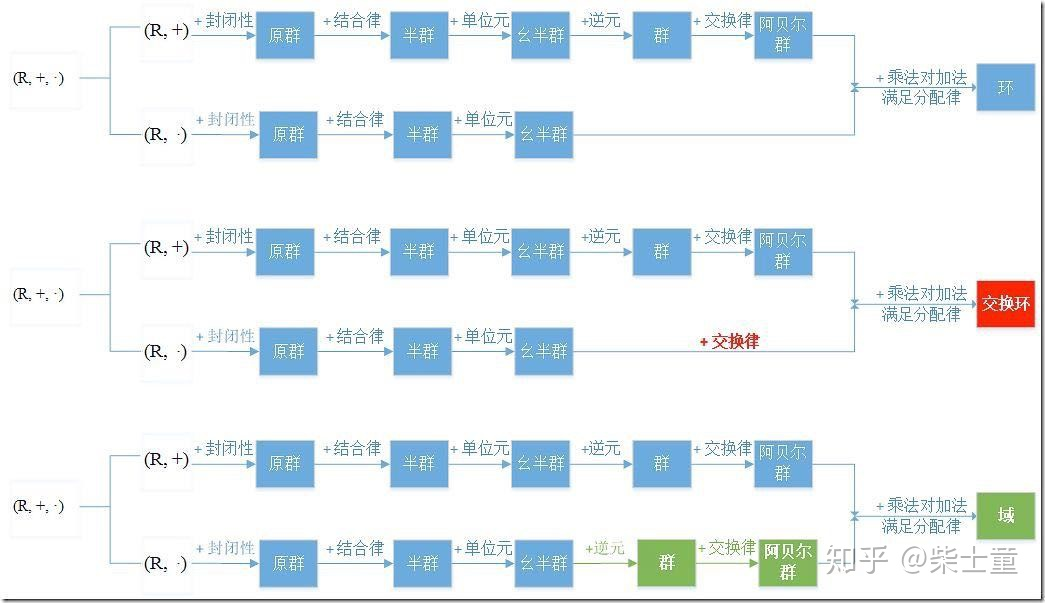
\includegraphics[width=1.0\textwidth]{fig/GroupRingField.jpg}
\end{figure}

\subsubsection{环(ring)}
环在阿贝尔群(也叫交换群)的基础上,添加一种二元运算·(虽叫乘法,但不同于初等代数的乘法)。一个代数结构是环$(R, +, ·)$,需要满足环公理(ring axioms)。环公理如下:
\begin{enumerate}
\setlength{\itemsep}{0pt}
\setlength{\parsep}{0pt}
\setlength{\parskip}{0pt}
\item $(R, +)$是交换群
	\begin{itemize}
	\setlength{\itemsep}{0pt}
	\setlength{\parsep}{0pt}
	\setlength{\parskip}{0pt}
	\item 封闭性:$a ∗ b$仍然属于该集合
	\item 结合律:$(a ∗ b) ∗ c = a ∗ (b ∗ c)$
	\item 单位元:$a ∗ e = a   \ \& \  e ∗ a = a$
	\item 逆元:加法的逆元为$-a$,乘法的逆元为倒数$1/a$,… (对于所有元素)
	\item 交换律:a + b = b + a
	\end{itemize}

\item $(R, ·)$是幺半群
	\begin{itemize}
	\setlength{\itemsep}{0pt}
	\setlength{\parsep}{0pt}
	\setlength{\parskip}{0pt}
	\item 结合律:$(a ⋅ b) ⋅ c = a ⋅ (b ⋅ c)$
	\item 单位元:乘法的单位元为1,$a * 1 = a   \ \& \  1 * a = a$
	\end{itemize}
	
\item 乘法对加法满足分配律
	\begin{itemize}
	\setlength{\itemsep}{0pt}
	\setlength{\parsep}{0pt}
	\setlength{\parskip}{0pt}
	\item $a ⋅ (b + c) = (a ⋅ b) + (a ⋅ c) \ \forall a, b, c \in R$
	\item $(b + c) ⋅ a = (b ⋅ a) + (c ⋅ a) \ \forall a, b, c \in R $
	\end{itemize}
\end{enumerate}

\subsubsection{交换环(commutative ring)}
交换环(commutative ring)在环的基础上,二元运算乘法还满足交换律。

\subsubsection{整环(integral domain)}
整环在交换环的基础上,并满足没有零因子(如此,集合内任意两个元素乘积均不等于0)

\subsection{域(Field)}
域(Field)在交换环的基础上,还增加了二元运算除法,要求元素(除零以外)可以作除法运算,即每个非零的元素都要有乘法逆元。由此可见,\textbf{域是一种可以进行加减乘除(除0以外)的代数结构,是数域与四则运算的推广}。整数集合,不存在乘法逆元(1/3不是整数),所以整数集合不是域;有理数、实数、复数可以形成域,分别叫有理数域、实数域、复数域。

\subsection{向量空间(vector space)}
向量空间是一些向量的集合。最熟悉的例子是几何向量或矢量(Euclidean vectors, geometric vector, spatial vector),表示具有大小和方向的对象;矢量可以做加法(addition)和乘法(scalar multiplication)运算

其他例子,还包括坐标空间(Coordinate spaces)、复数、函数空间(Function spaces)、线性方程组(linear equations)。

\section{群与代数}
\subsection{整数集合与同余关系}
待整理

\subsection{算数基本定理与欧拉函数}
待整理


%\printbibliography
\bibliography{../ref}
\bibliographystyle{IEEEtran}
\end{document}
